\PassOptionsToPackage{table}{xcolor}
\documentclass[12pt,a4paper]{article}

\usepackage{iftex}
\ifPDFTeX
  \usepackage[T1]{fontenc}
  \usepackage[utf8]{inputenc}
\else
  \usepackage{fontspec}
\fi
\usepackage[turkish]{babel}
\usepackage[margin=2.4cm]{geometry}
\usepackage{setspace}
\usepackage{graphicx}
\usepackage{booktabs}
\usepackage{longtable}
\usepackage{array}
\usepackage{colortbl}
\usepackage{xcolor}
\usepackage{enumitem}
\usepackage{listings}
\usepackage{amssymb}
\usepackage{caption}
\usepackage{fancyhdr}
\usepackage{hyperref}
\usepackage{xurl}
\setlength{\headheight}{15pt}
\graphicspath{{rapor-gorseller/}}

\onehalfspacing
\setlength{\parindent}{0pt}
\setlength{\parskip}{6pt}
\setlist{itemsep=2pt, topsep=4pt}
\hypersetup{colorlinks=true, linkcolor=blue!50!black, urlcolor=blue!50!black}

\definecolor{ana}{HTML}{14325C}
\definecolor{acik}{HTML}{EEF2F8}

\lstset{basicstyle=\ttfamily\small, backgroundcolor=\color{acik},
  frame=single, rulecolor=\color{ana}, breaklines=true,
  columns=fullflexible, keepspaces=true, showstringspaces=false}

\pagestyle{fancy}
\fancyhf{}
\fancyhead[L]{Kayıp Rıhtım}
\fancyhead[R]{Vize Raporu}
\fancyfoot[C]{\thepage}

\newcommand{\aciklama}[1]{{\color{gray}\itshape (#1)}}

\newcommand{\haftagorsel}[1]{%
  \IfFileExists{rapor-gorseller/#1}{%
    \includegraphics[width=\linewidth,height=4.2cm,keepaspectratio]{rapor-gorseller/#1}%
  }{%
    \fbox{\parbox[c][2.6cm][c]{\dimexpr\linewidth-2\fboxsep-2\fboxrule\relax}{%
      \centering\small\color{gray} Ekran görüntüsü / görsel ekleyin\\ \texttt{#1}}}%
  }%
}
\newcommand{\katilimkutulari}{\par\vspace{3pt}\small $\square$ Ders içinde katılım sergiledim\par $\square$ Telafi yaptım}

\newcommand{\haftaek}[1]{%
  \IfFileExists{rapor-gorseller/#1}{\\[4pt]\includegraphics[width=\linewidth,height=4.2cm,keepaspectratio]{rapor-gorseller/#1}}{}%
}

\newcommand{\universite}{İstanbul Medipol Üniversitesi / Görsel İletişim Tasarımı}
\newcommand{\dersadi}{Programlamaya Giriş}
\newcommand{\hocaadi}{Meral Şentürk}
\newcommand{\ogrenciadi}{Özcan Atiş}
\newcommand{\ogrencino}{86240023}
\newcommand{\projeadi}{Kayıp Rıhtım}
\newcommand{\githublink}{\url{https://github.com/ozcan857/kayip-rihtim}}
\newcommand{\youtubelink}{\url{https://youtu.be/AQAaNiV5dAc}}

\begin{document}
\shorthandoff{=!:}

\begin{titlepage}
\centering
\vspace*{1cm}
{\large \universite \par}
\vspace{1.8cm}
{\Huge\bfseries\color{ana} \projeadi \par}
\vspace{0.4cm}
{\Large Türk Masalları Derlemesi Web Sayfası \par}
{\large Vize Raporu \par}
\vspace{1.8cm}
{\large \textbf{Ders:} \dersadi \par}
{\large \textbf{Öğretim Üyesi:} \hocaadi \par}
\vspace{1.2cm}
{\large \textbf{Hazırlayan:} \ogrenciadi \par}
{\large \textbf{Öğrenci No:} \ogrencino \par}
\vspace{1.8cm}
\fbox{\parbox{0.88\linewidth}{\centering\vspace{6pt}
{\large\bfseries Proje Bağlantıları}\\[8pt]
\textbf{GitHub deposu:}\\ \githublink \\[8pt]
\textbf{YouTube sunum videosu:}\\ \youtubelink
\vspace{6pt}}}
\vfill
{\large 6 Kasım 2026 \par}
\end{titlepage}

\tableofcontents
\newpage

\section{Giriş}


\subsection{Proje Özeti}
Kayıp Rıhtım, Türk halk anlatılarına ilgi duyan genel okuyucular için hazırlanmış bir masal okuma sitesidir. Seçkide sekiz masalın tam metni bulunur. Projede içerik seçimini kolaylaştıran bir ana liste ile metne odaklanan ortak bir okuma alanı tasarladım. Okuyucunun tercihine göre gündüz, sepya ve gece temaları ile yazı boyutu ayarı ekledim.

\subsection{Gereksinimlerin Karşılanması}
\begin{center}
\rowcolors{2}{acik}{white}
\begin{tabular}{@{}p{8.2cm}c@{}}
\toprule
\rowcolor{ana}\textcolor{white}{\textbf{Gereksinim}} & \textcolor{white}{\textbf{Durum}} \\
\midrule
Masal sayısı 8--12 arasında (8 masal)         & $\boxtimes$ \\
Tek HTML dosyası                                    & $\boxtimes$ \\
Stil kodları içsel (\texttt{<style>} içinde)        & $\boxtimes$ \\
Betik kodları içsel (\texttt{<script>} içinde)      & $\boxtimes$ \\
İnternetsiz açılıp çalışıyor                        & $\boxtimes$ \\
JavaScript sayfada anlamlı bir işlev görüyor        & $\boxtimes$ \\
Sayfa telefonda da düzgün görünüyor                 & $\boxtimes$ \\
\bottomrule
\end{tabular}
\end{center}


\section{Masalların Seçimi}

Sekiz masalı seçerken olabildiğince farklı tonları bir araya getirmeye çalıştım. Kartların üzerinde yer alan sabır, korku, sevgi, cesaret ve özgürlük gibi anahtar kelimeler, her masalın genel vurgusunu anlatıyor. Bu etiketleri hem ana listede hem okuma ekranında kullanarak seçilen masalın temasını takip edilebilir tuttum. Siteyi çocuklara özel hazırlamadığım için metinleri pedagojik bir uyarlama amacıyla yumuşatmadım. Seçimimde genel okuyucuya sunulabilecek anlatı çeşitliliği ön plandaydı.


\begin{longtable}{@{}cp{3.5cm}p{2.6cm}p{5.5cm}@{}}
\toprule
\textbf{No} & \textbf{Masal} & \textbf{Tür} & \textbf{Seçilme nedeni} \\
\midrule
\endhead
1 & Dört Öğüt & Öğüt masalı & Sabır ve karar verme temasını seçkiye katması. \\
2 & Kurnaz Kurt & Hayvan masalı & Korku ve kurnazlık üzerinden farklı bir anlatım sunması. \\
3 & Tuz Kadar Sevgi & Olağanüstü masal & Sevgi ve değer kavramlarını gündelik bir nesneyle ilişkilendirmesi. \\
4 & Korkak Adam ve Devler & Dev masalı & Güç karşısında zekâ ve yanıltma temasını işlemesi. \\
5 & Nardaniye Hanım & Olağanüstü masal & Tehlike, sığınma ve kimlik etrafında gelişen olay örgüsü. \\
6 & Üç Turunçlar & Olağanüstü masal & Dönüşüm ve arayış motifleriyle anlatı çeşitliliği sağlaması. \\
7 & Ali Cengiz Oyunu & Olağanüstü masal & Usta-çırak ilişkisi ve dönüşüm motifini işlemesi. \\
8 & Keloğlan ve Altın Bülbül & Olağanüstü masal & Yolculuk, azim ve gerçeğin ortaya çıkması temaları. \\
\bottomrule
\end{longtable}

\section{Tasarım Kararları}


\subsection{Konuya Uygunluk}
İçerik çocuklara özel olmadığı için tasarımı da çocuklara yönelik bir görsel dille kurmak istemedim. Kitap sayfasını çağrıştıran, metin ağırlıklı ve sade bir görünüm tercih ettim. Son sürümde masal içi görselleri kaldırdım. ``Kayıp Rıhtım'' adını, fantastik edebiyat alanında tanıdığım aynı adlı oluşuma bir gönderme olarak seçtim; proje bu oluşumun resmî bir çalışması değildir. Sitenin adını taşıyan bağlantı ile tema seçimini üst şeritte topladım. Sepya temadaki krem zemin ve bordo vurgular, bu sade okuma görünümünü tamamlıyor.

\subsection{Renk Paleti ve Yazı Tipi}
Masalın gövde metninde ve büyük başlıklarda Georgia, yardımcı arayüz yazılarında Arial kullandım. Georgia tercihimde ekranda uzun metin okumaya uygun bir kitap görünümü elde etme isteği etkili oldu. Fontları internetten indirmek yerine cihazda bulunan yazı tiplerini kullanacak bir sıra tanımladım; Georgia veya Arial bulunmadığında listedeki yedekler devreye giriyor. Gündüz, sepya ve gece seçeneklerini de tek bir renk düzenini zorunlu tutmamak, okuyucuya tercih sunmak için ekledim.

\begin{center}
\rowcolors{2}{acik}{white}
\begin{tabular}{@{}llp{6.4cm}@{}}
\toprule
\rowcolor{ana}\textcolor{white}{\textbf{Ad}} & \textcolor{white}{\textbf{Kod}} & \textcolor{white}{\textbf{Nerede / neden kullandınız?}} \\
\midrule
Krem zemin & \texttt{\#F6F0E4} & Sepya temada kâğıt çağrışımı yapan ana zemin. \\
Koyu kahve & \texttt{\#302C27} & Sepya temanın temel metin rengi. \\
Bordo & \texttt{\#79382F} & Bağlantılar, vurgu yazıları ve ilk harf. \\
Yeşil & \texttt{\#4C5E4E} & Kartlardaki tema etiketleri. \\
Georgia & Serif & Masal metni ve büyük başlıklar; bulunmazsa serif yedekler. \\
Arial & Sans-serif & Arayüz metinleri; Helvetica ve genel sans-serif yedekleri. \\
\bottomrule
\end{tabular}
\end{center}

\subsection{Okunabilirlik, Gezinme ve Duyarlı Tasarım}
\begin{itemize}
  \item \textbf{Okunabilirlik:} Obsidian gibi not alma uygulamalarında kullandığım, ekranın tamamına yayılmayan metin sütununu örnek aldım. Geniş bilgisayar ekranlarında satırların fazla uzamasını istemedim; okuma alanını en çok 740 px ile sınırlayıp sağında ve solunda boşluk bıraktım. Ortalanan şey sütundur; paragraf satırları sola hizalıdır. Başlangıç yazı boyutu 21 px, satır yüksekliği 1.72'dir. Okuyucu boyutu 2 px adımlarla değiştirebilir; son koddaki sınırlar 14 ve 29 px'tir. Bu tercihleri bütün okuyucular için geçerli bir sağlık veya göz yorgunluğunu önleme iddiası olarak sunmuyorum.
  \item \textbf{Gezinme:} Ana sayfada masallar iki sütun hâlinde listelenir. Kartların üzerine imleç geldiğinde zeminin aydınlanması ve hafif gölge oluşması, o alanın tıklanabildiğini belirtir. Okuma ekranında ana listeye dönüş bağlantısı ve kaçıncı masalda olunduğunu gösteren bilgi bulunur. Kaynaklar açılır kapanır bir alanda gösterilir. En alttaki bağlantılarla varsa önceki veya sonraki masala geçilebilir.
  \item \textbf{Duyarlı tasarım:} 520 px ve altındaki görüntüleme alanlarında masal listesi tek sütuna iner. Üst şerit sığmadığında alt satıra geçebilir; küçük tema noktaları gizlenir. Gerçek fiziksel telefonda yapılan bir test beyan etmiyorum.
  \item \textbf{Tutarlılık:} Ana listedeki tema etiketi, masalın başlığı ve kısa tanıtımı okuma ekranında da devam eder. Ortak sınıflar, renk değişkenleri ve aynı kart yapısı bütün masallarda kullanılır. Sayfanın sonundaki ``Gökten üç elma düşmüş'' ifadesini tanıdık bir masal kapanışı olarak kullandım.
\end{itemize}

\subsection{Ekran Görüntüleri}
\begin{figure}[htbp]
\centering
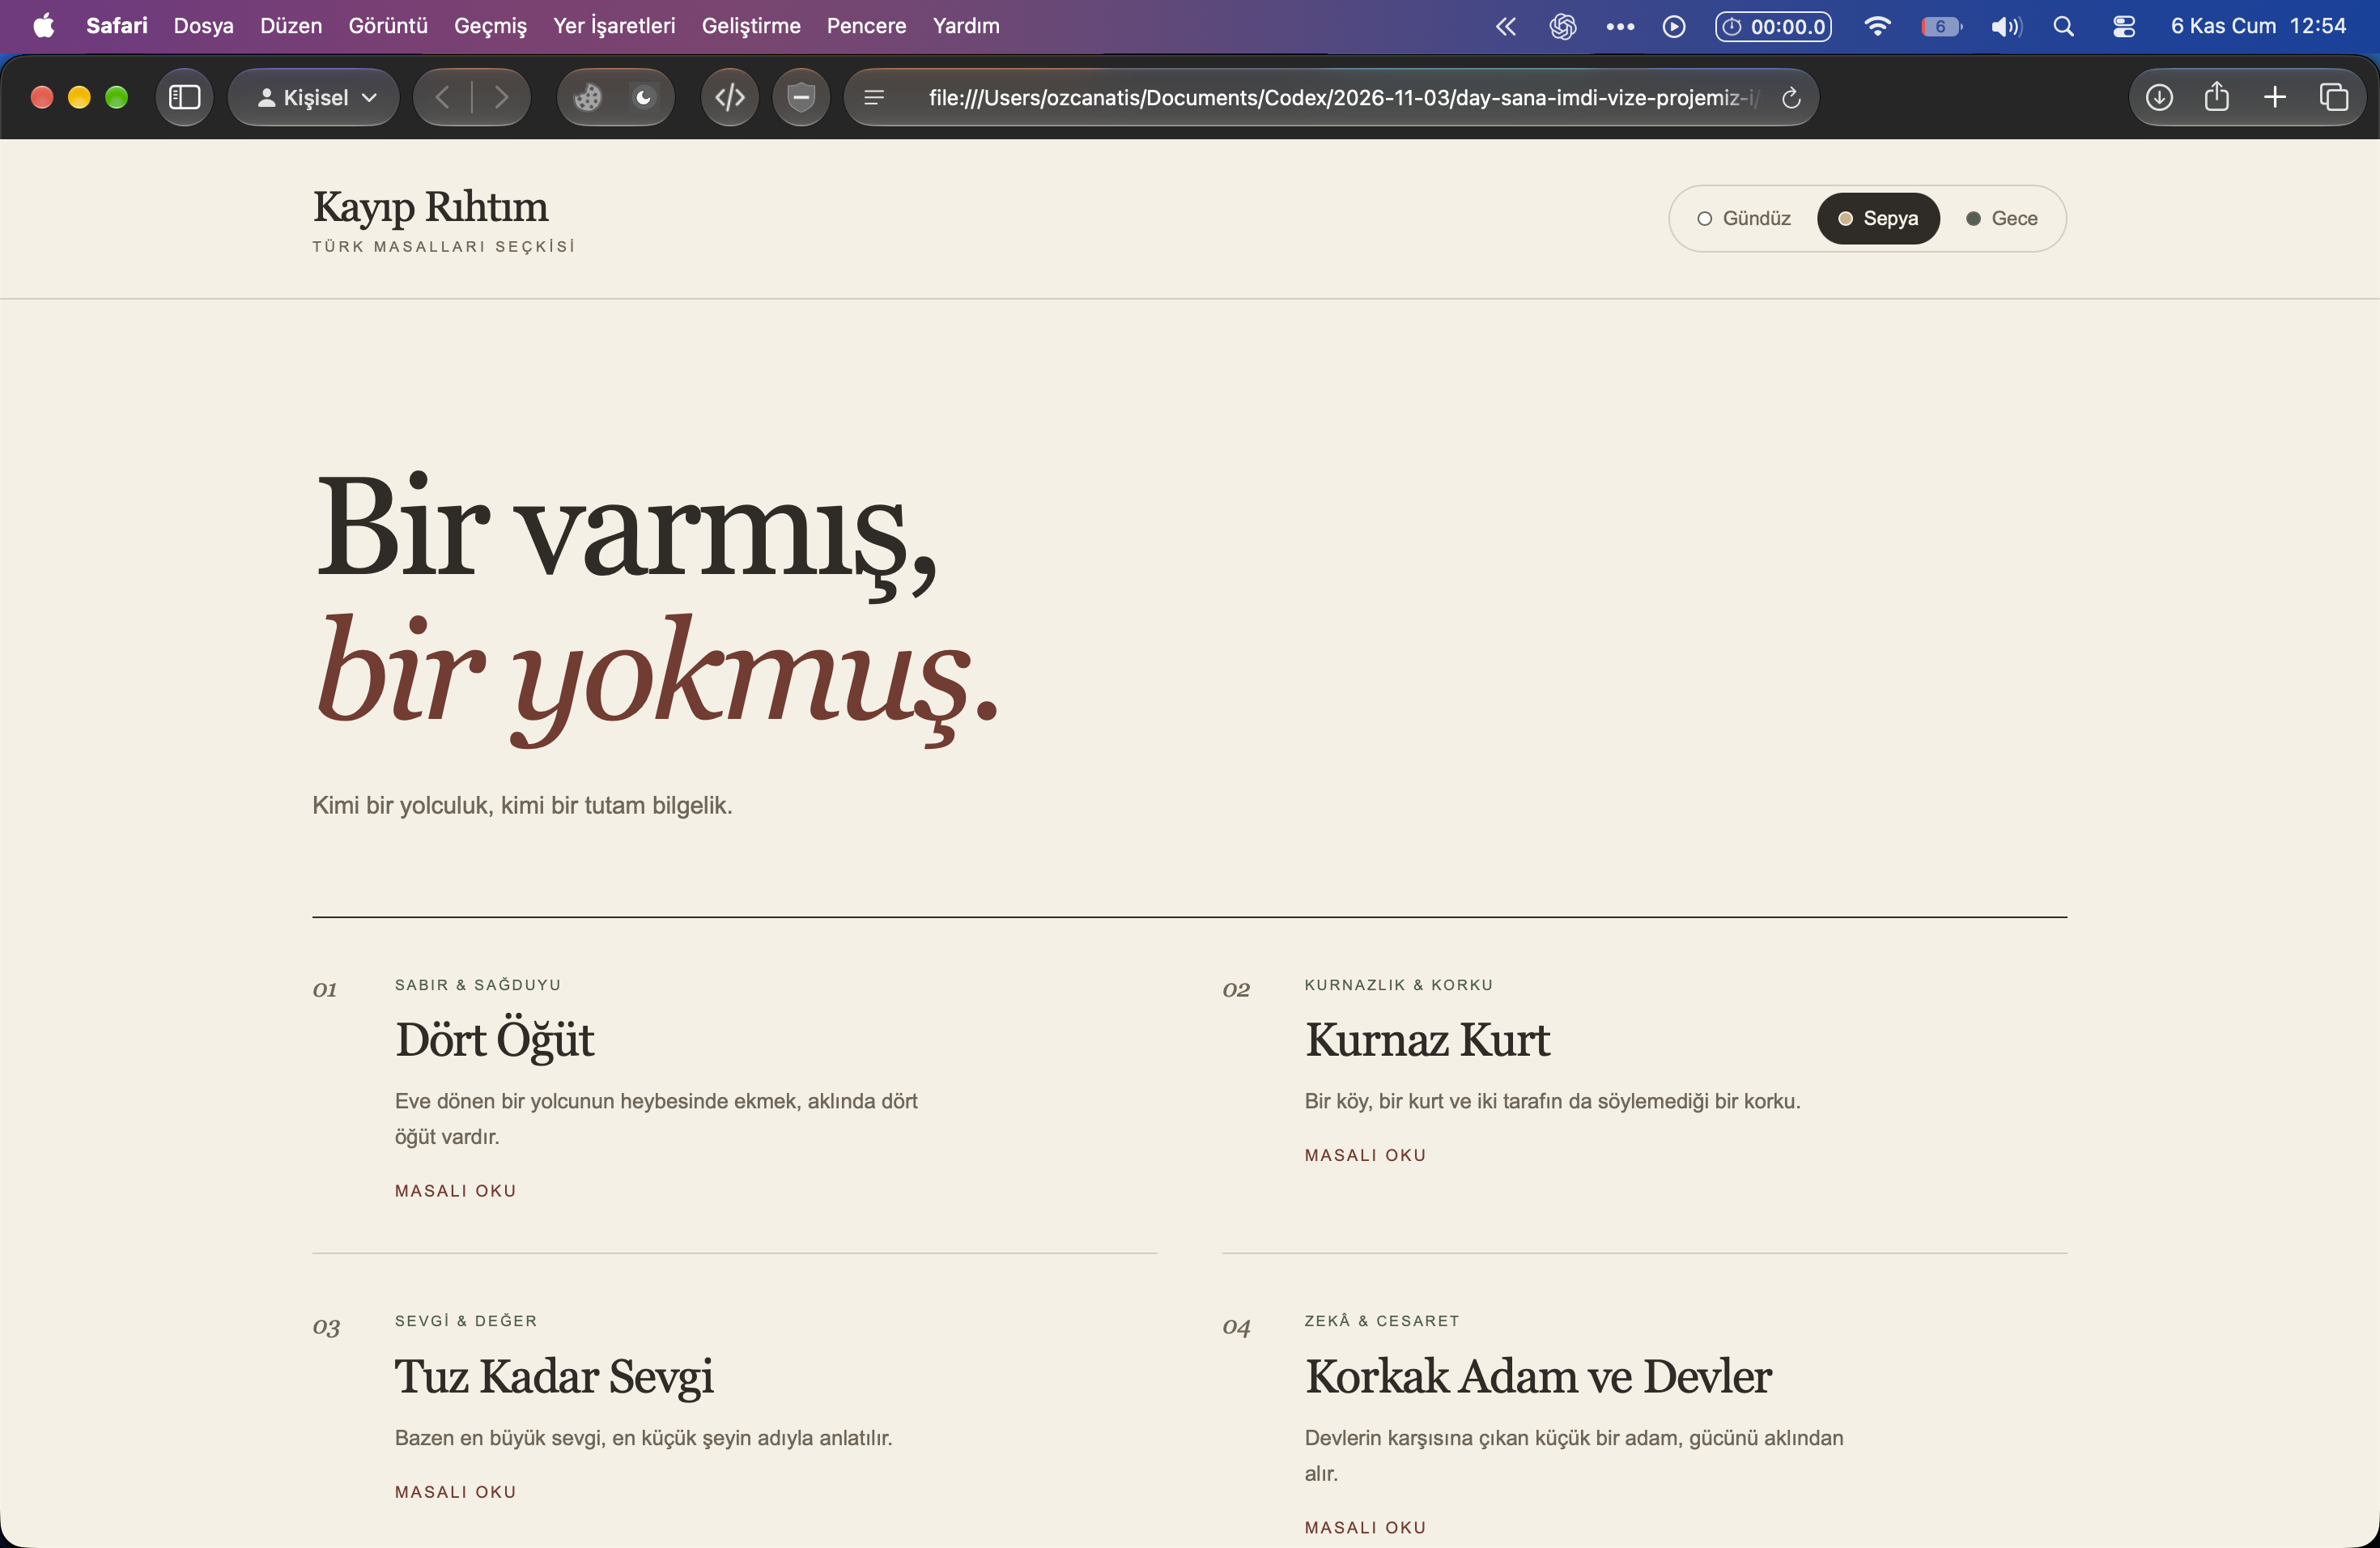
\includegraphics[width=.95\linewidth,height=.64\textheight,keepaspectratio]{site-anasayfa.png}
\caption{Sepya temada ana sayfa ve iki sütunlu masal listesi}
\end{figure}
\begin{figure}[htbp]
\centering
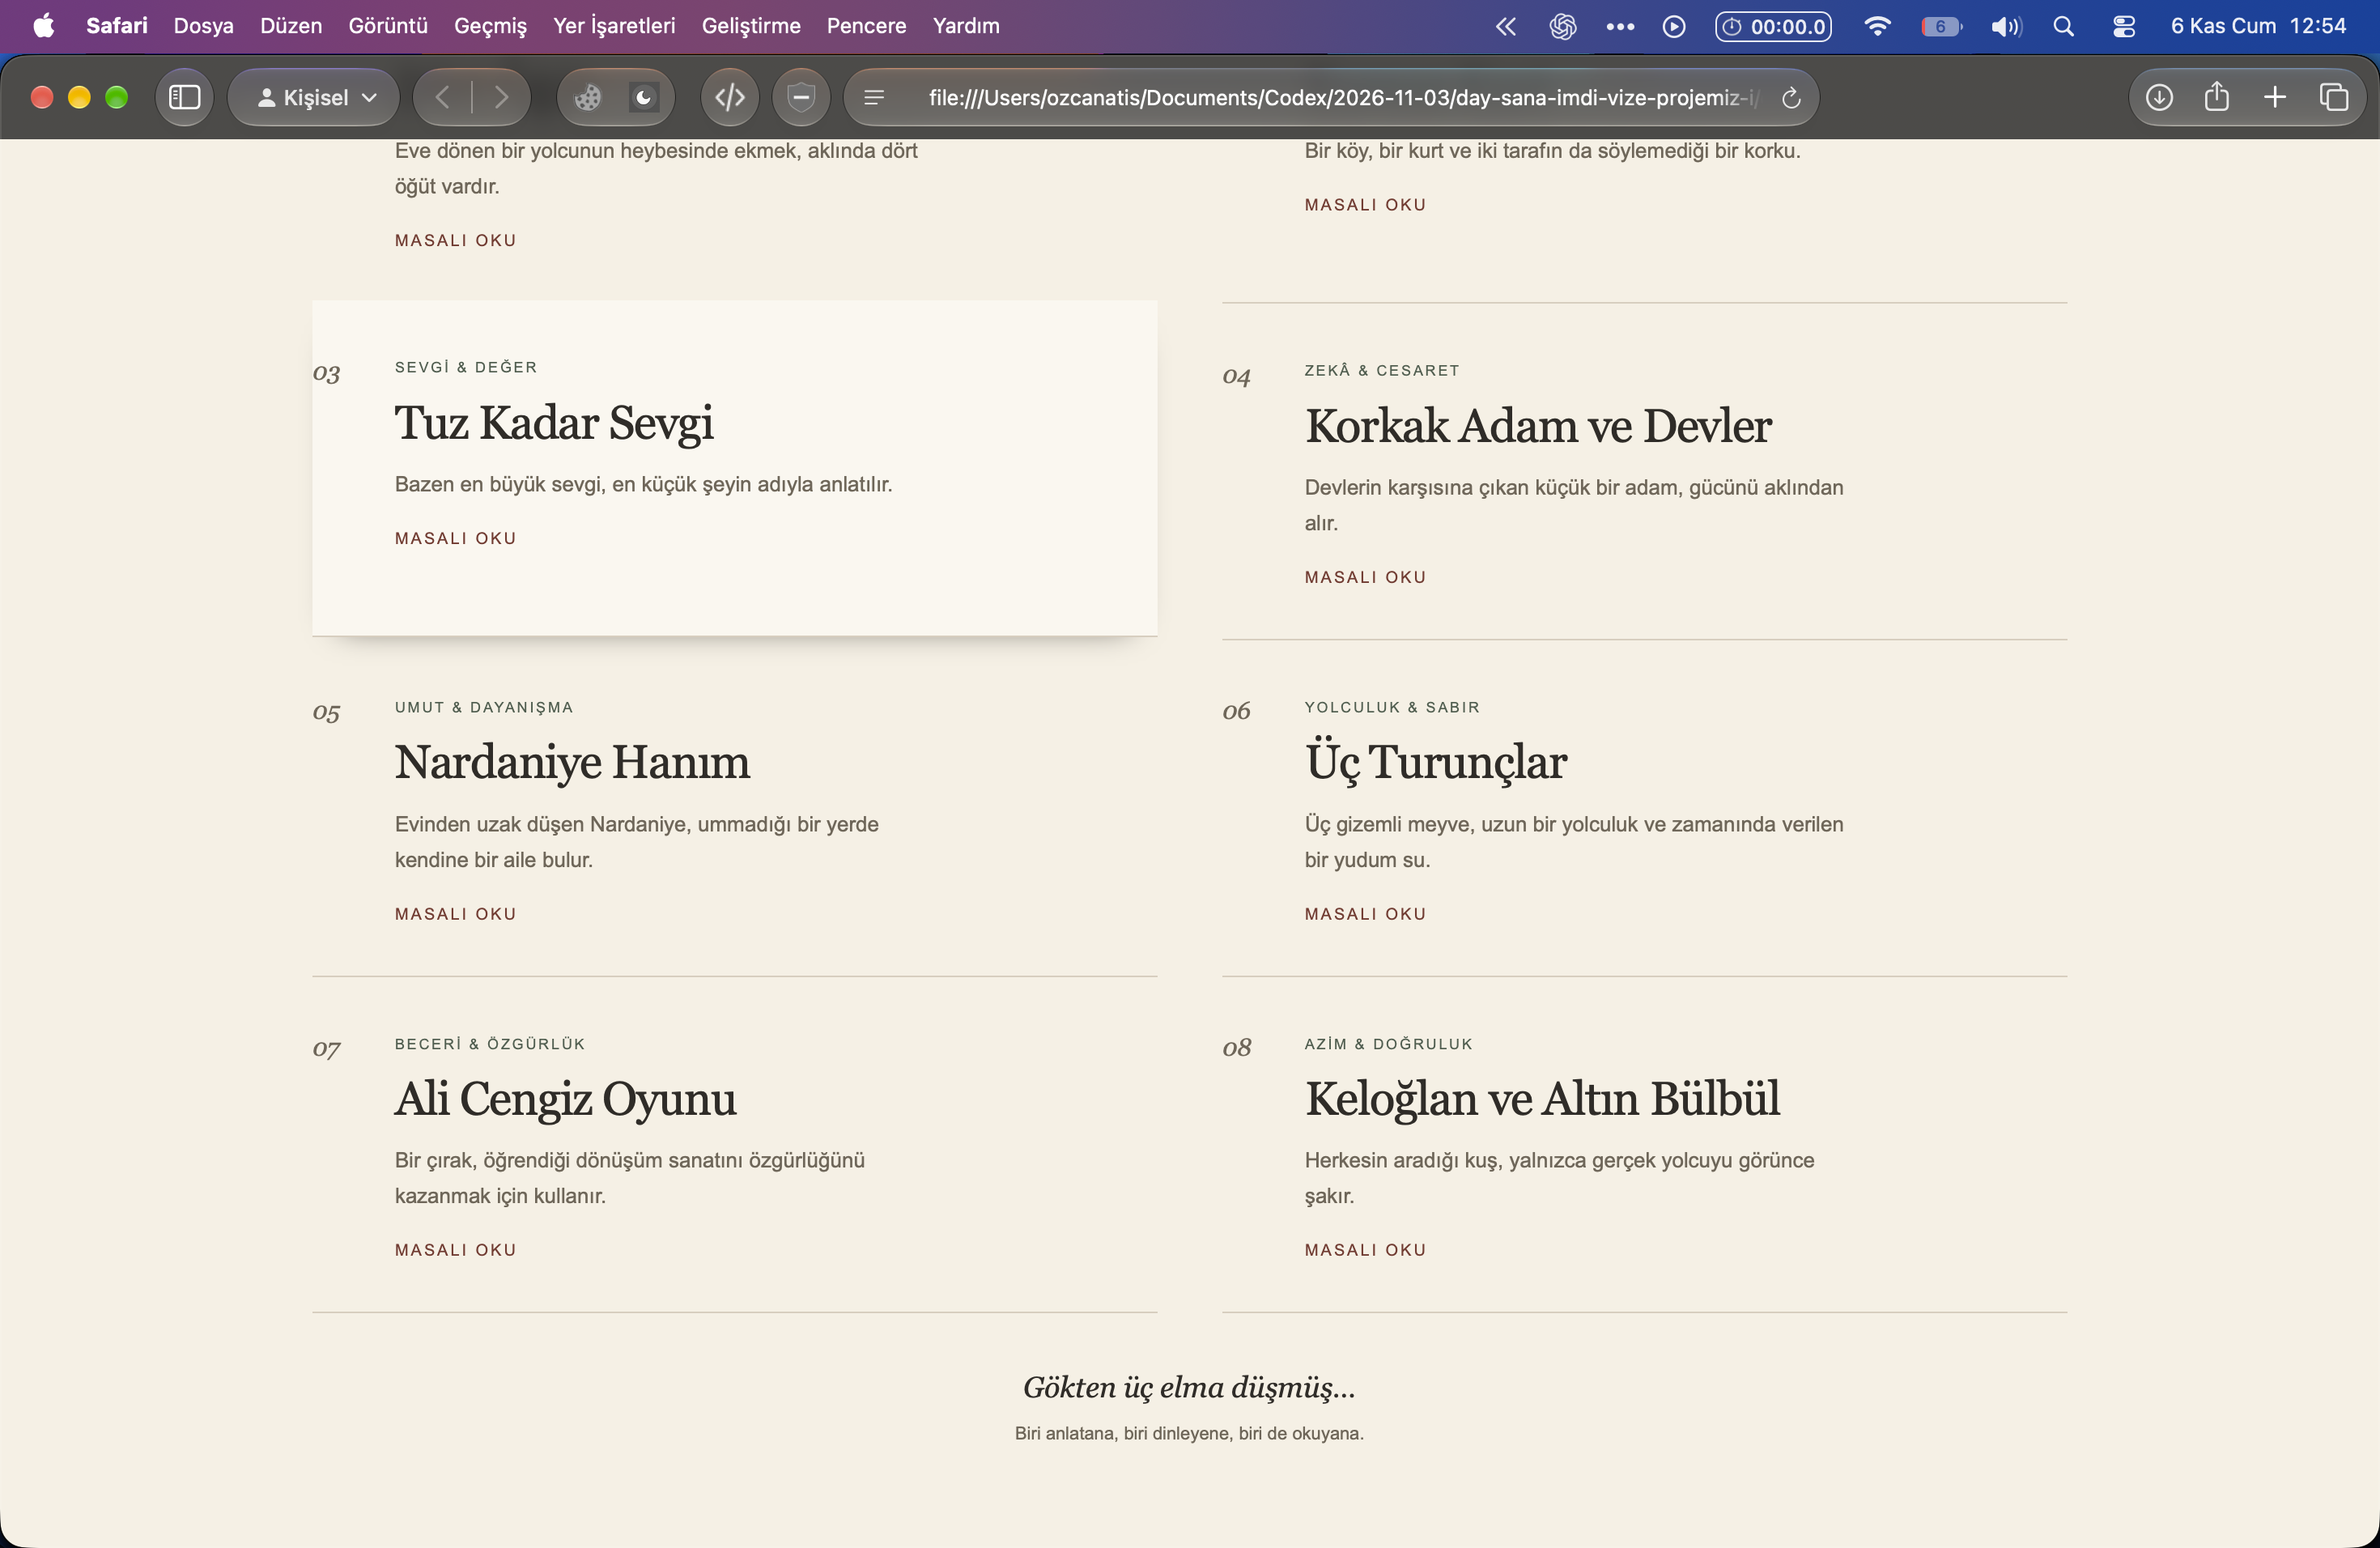
\includegraphics[width=.95\linewidth,height=.64\textheight,keepaspectratio]{site-kartlar.png}
\caption{Masal kartları, üzerine gelme vurgusu ve seçkinin kapanışı}
\end{figure}
\begin{figure}[htbp]
\centering
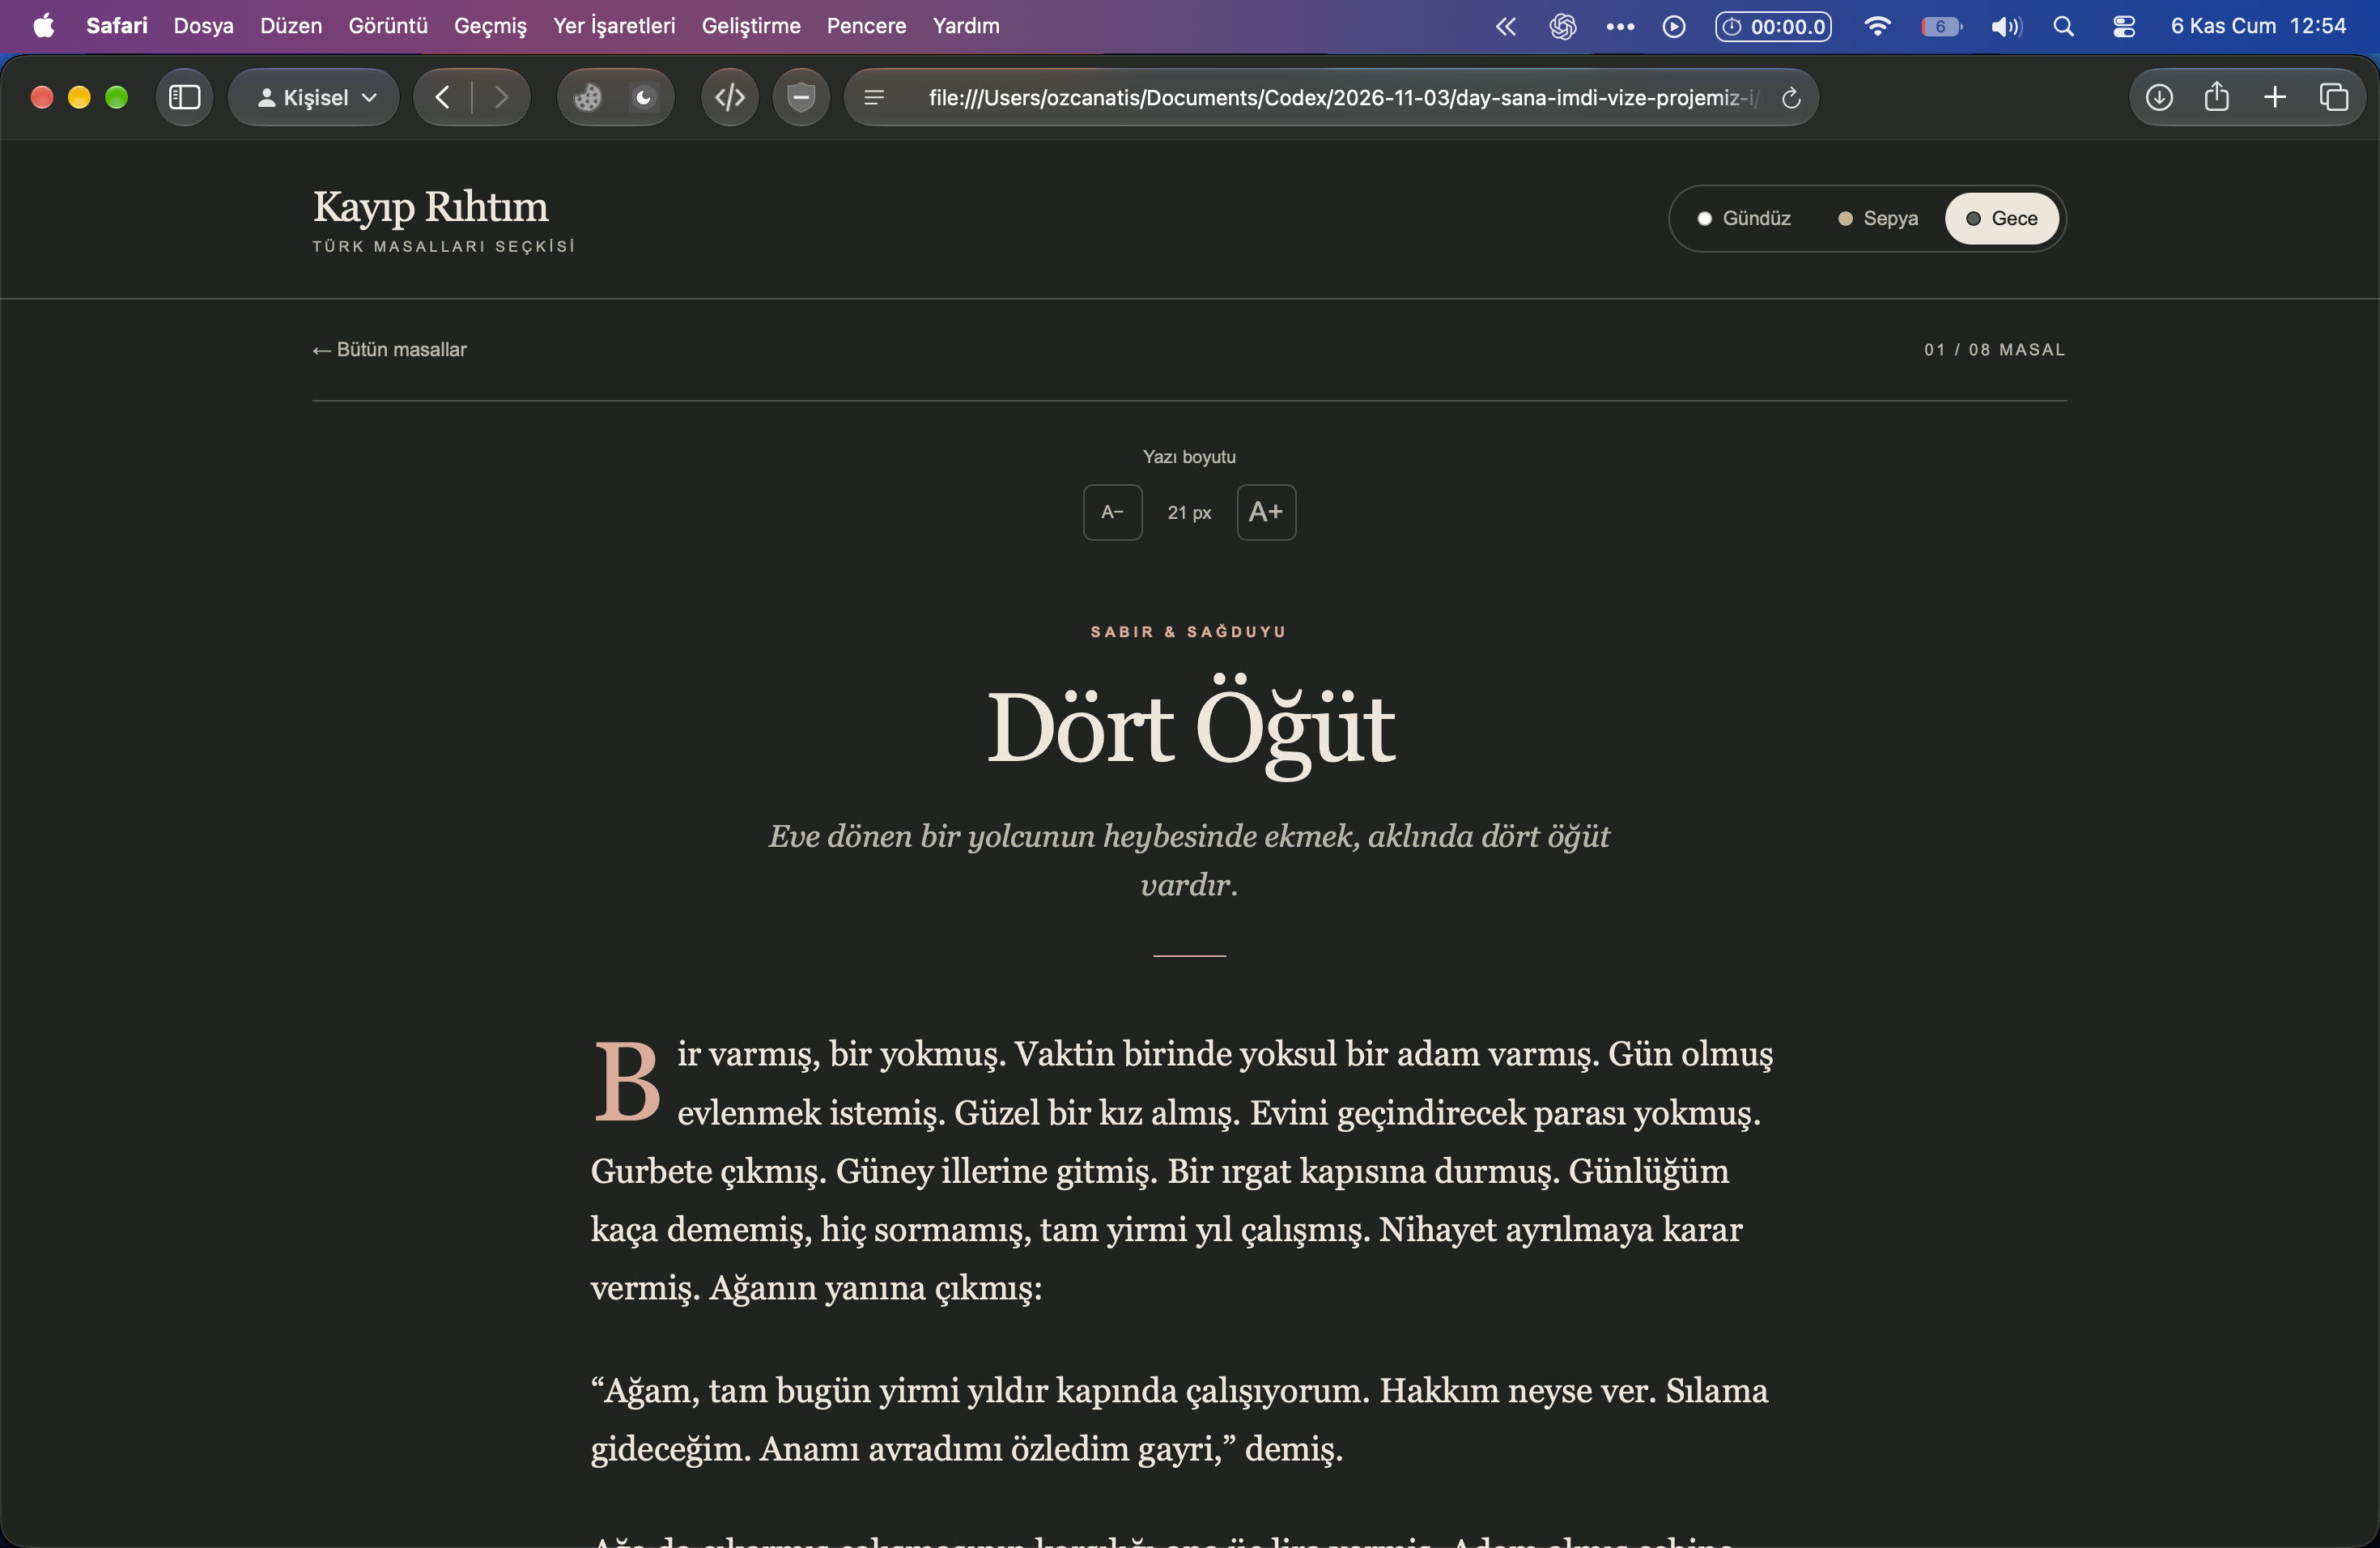
\includegraphics[width=.95\linewidth,height=.64\textheight,keepaspectratio]{site-gece-okuma.png}
\caption{Gece modunda Dört Öğüt: yazı boyutu ayarı ve okuma sütunu}
\end{figure}
\clearpage

\section{Gerçekleştirme}


\subsection{HTML Yapısı}
Üst şeritte \texttt{header}, ana içerikte \texttt{main}, seçki ve okuma alanlarında \texttt{section} kullandım. Okunan masal \texttt{article} içinde gösterilir. Masal başlığı, tema yazısı ve paragraflar için kimliği belirlenmiş boş elemanlar bulunur; JavaScript seçilen masala göre bunları doldurur. Kaynak bilgisi \texttt{details} ve \texttt{summary} etiketleriyle açılır kapanır biçimde sunulur. Okuma alanı başlangıçta \texttt{hidden} özelliğiyle gizlidir. Ayrı HTML sayfaları yerine aynı belgedeki iki görünüm arasında geçiş yapılır.

\subsection{İçsel CSS}
CSS kodu HTML dosyasındaki \texttt{style} etiketi içinde yer alır. Renkler \texttt{--paper}, \texttt{--ink} ve \texttt{--accent} gibi değişkenlerde tutulur. Tema seçimi, \texttt{html} elemanının \texttt{data-theme} bilgisine göre bu renkleri değiştirir. Üst şerit ve düğmelerde Flexbox, masal kartlarında Grid kullandım. Kartların üzerine gelindiğinde hafif gölge, zemin değişimi ve 2 px yukarı hareket tıklanabilirliği belirtir. Masalın ilk harfi \texttt{::first-letter} ile büyütülür. Sınıf adlarını kodu takip etmeyi kolaylaştırmak amacıyla Türkçe ve ASCII karakterlerle adlandırdım.

Sunumda bazı değerleri değiştirerek sonuçlarını gösterdim. Üst şeridin alt çizgisini 1 px'ten 5 px'e çıkarmak çizgiyi kalınlaştırır. Başlıktaki \texttt{br} kaldırılırsa zorunlu satır kırılması kalkar. Grid düzeninde \texttt{1fr 1fr} yerine üç kez \texttt{1fr} yazmak üç eşit sütun oluşturur; \texttt{column-gap} ise sütunlar arasındaki boşluğu değiştirir. Başlığın boyutunu değiştirmek için CSS'teki yazı boyutu kullanılmalıdır; \texttt{h1} ve \texttt{h2} etiketleri başlık hiyerarşisini belirtir. CSS değişkenlerinde aynı renk ve ölçüleri isimle tekrar kullanmak, düzenlemeyi daha kolay takip etmemi sağladı.

\begin{lstlisting}[caption={İçsel CSS'ten önemli bir bölüm}]
.okuma-alani {
  max-width: 740px;
  margin: 0 auto;
  padding: 45px 0 65px;
}
.masal-listesi {
  display: grid;
  grid-template-columns: 1fr 1fr;
  column-gap: 40px;
}
@media (max-width: 520px) {
  .masal-listesi { grid-template-columns: 1fr; }
}
\end{lstlisting}

\subsection{İçsel JavaScript}
Masallar \texttt{stories} dizisindeki nesnelerde saklanır. Her nesnede kimlik, başlık, kısa tanıtım, paragraf listesi ve kaynak bilgileri bulunur. \texttt{forEach} ile masal kartları oluşturulur. \texttt{route()} adresin hash bölümünü okuyarak seçilen masalı bulur; \texttt{showStory()} ortak okuma alanını doldurur. \texttt{hashchange} olayı görünümü günceller. Düğmelere \texttt{addEventListener} ile tıklama olayları bağlanır. \texttt{settings} nesnesindeki tema ve boyut değerlerini \texttt{applySettings()} CSS değişkenlerine ve düğmelerin seçili durumlarına uygular. Sadeleştirilmiş son sürümde ayarlar kalıcı depolamaya yazılmaz; kod yeniden çalıştığında başlangıç değerleri kullanılır.

Videoda site adına tıklanınca Dört Öğüt'ün açılmasını da bağlantının \texttt{href} değerini değiştirerek denedim. Masal kartlarının adresleri, \texttt{\#masal/} metnine ilgili masalın kimliği eklenerek oluşur. Tema düğmeleri aynı sınıfı paylaşır; gündüz, sepya ve gece seçeneklerini birbirinden ayıran bilgi \texttt{data-value} değeridir.

Yazı boyutunun alt sınırını değiştirirken iki ayrı noktayı birlikte düşünmem gerektiğini gördüm. \texttt{Math.max} değeri sayısal sınırı belirlerken \texttt{disabled} kontrolü düğmenin ne zaman kullanılamaz olacağını belirler. Videoda 10 px sınırını bir deneme olarak gösterdim; teslim dosyasındaki alt sınır 14 px'tir. CSS'te kullandığım birim px'tir; tipografik puntoyu ifade eden pt ile aynı birim değildir.

\begin{lstlisting}[caption={İçsel JavaScript'ten önemli bir bölüm}]
const settings = {theme: 'sepia', size: 21};
document.querySelectorAll('.tema-dugmesi').forEach(button => {
  button.addEventListener('click', () => {
    settings.theme = button.dataset.value;
    applySettings();
  });
});
window.addEventListener('hashchange', route);
\end{lstlisting}

\subsection{Sayfanın Özellikleri}
Sekiz tam masal metni, üç okuma teması, yazı boyutu ayarı, ana listeye dönüş ve masallar arasında gezinme bulunur. Her masalın altında ayrı kaynak bilgisi vardır. Çevrimdışı kullanım için harici yazı tipi, kütüphane, görsel veya veri isteğine bağımlılık yoktur. Dış kaynak bağlantıları ise internet gerektirir. Kullanılmayan genel hakkında bölümü son sürümden kaldırılmıştır.


\section{Yapay Zekâ Kullanımı}


\begin{longtable}{@{}p{2.1cm}p{3cm}p{4cm}p{3cm}@{}}
\toprule
\textbf{Araç} & \textbf{Ne için kullandınız?} & \textbf{İstem (prompt) özeti} & \textbf{Sayfada nerede?} \\
\midrule
\endhead
Codex / ChatGPT & Kod, düzenleme ve öğrenme desteği & Tek HTML içinde masal listesi, okuma temaları, yazı boyutu ve hash ile gezinme; kodların temel açıklamaları. & HTML, CSS, JavaScript ve rapor hazırlığı. \\
Adobe Firefly & Görsel denemeleri & Masal sahneleri için çizim ve şeffaf arka plan denemeleri. & Son sitede kullanılmadı. \\
\bottomrule
\end{longtable}

\subsection{Anladığım ve Kendim Yaptığım Kısımlar}
Masalları farklı temaları bir araya getirecek biçimde seçtim. Genel okuyucuya yönelik olmasına, adına, görsel kullanılmamasına ve okuma sütununun yerleşimine karar verdim. Kod desteği için Codex kullandım; aldığım kodları daha rahat takip edebilmek için sadeleştirmeye çalıştım. Hazır örneği yalnızca izlemek yerine CodePen'de çizgi kalınlığı, sütun sayısı, renk ve yazı boyutu gibi değerleri değiştirip sonuçlarını gözlemledim. Sınıf adlarının bizim seçtiğimiz isimler olduğunu, kimliklerin JavaScript ile elemanlara erişmede kullanıldığını ve tıklama olaylarının işleyişini çalıştım. Sunum videosunu kendim kaydettim.

\section{Haftalık Katkılar}


\begin{longtable}{@{}>{\raggedright\arraybackslash}p{1.7cm}%
                    >{\raggedright\arraybackslash}p{6cm}%
                    >{\centering\arraybackslash}p{5.3cm}@{}}
\toprule
\rowcolor{ana}\textcolor{white}{\textbf{Hafta}} & \textcolor{white}{\textbf{Yapılan çalışma}} & \textcolor{white}{\textbf{Görsel}} \\
\midrule
\endfirsthead
\toprule
\rowcolor{ana}\textcolor{white}{\textbf{Hafta}} & \textcolor{white}{\textbf{Yapılan çalışma}} & \textcolor{white}{\textbf{Görsel}} \\
\midrule
\endhead
\bottomrule
\endfoot

\textbf{1. hafta}\newline Ortak telafi; görsel tarihi 12.10.2026 & İlk iki haftanın ortak telafisi kapsamında WorldWideWeb temalı bir HTML sayfası hazırladım. Başlık, paragraf, liste ve sayfa içi bağlantıları kullandım; renk, yazı tipi ve boşlukları CSS ile düzenledim. Aynı ortak çalışmanın ilk kısmı burada gösterilmiştir.\par\textbf{Commit:} Bu çalışma için döneminde GitHub commit kaydı oluşturulmadı.\par\small $\square$ Ders içinde katılım sergiledim\par $\boxtimes$ Telafi yaptım & \haftagorsel{telafi-ust.png} \\
\midrule
\textbf{2. hafta}\newline Ortak telafi; görsel tarihi 12.10.2026 & Birinci haftayla ortak telafi çalışmasının devamıdır; ayrı bir ikinci proje değildir. Sayfa içi bağlantılar, alt başlıklar, yatay çizgi, adres alanı ve açıklama kutusu üzerinde çalıştım. Ortak çalışmanın alt kısmı burada gösterilmiştir.\par\textbf{Commit:} Bu çalışma için döneminde GitHub commit kaydı oluşturulmadı.\par\small $\square$ Ders içinde katılım sergiledim\par $\boxtimes$ Telafi yaptım & \haftagorsel{telafi-alt.png} \\
\midrule
\textbf{3. hafta}\newline 30.09.2026 & Düğmeye tıklandığında alert ile mesaj gösterdim. Tıklamayı onclick ve addEventListener ile tanımladım; bağlantıları aynı ve yeni sekmede açma örnekleri hazırladım.\par\textbf{Commit:} Bu çalışma için döneminde GitHub commit kaydı oluşturulmadı.\par\small $\boxtimes$ Ders içinde katılım sergiledim\par $\square$ Telafi yaptım & \haftagorsel{eylul30-uyari.png} \\
\midrule
\textbf{4. hafta}\newline 07.10.2026 & Düğmeye tıklanınca textContent ile mesaj yazdırdım. Artırma, azaltma ve sıfırlama düğmeleriyle çalışan bir sayaç oluşturdum.\par\textbf{Commit:} Bu çalışma için döneminde GitHub commit kaydı oluşturulmadı.\par\small $\boxtimes$ Ders içinde katılım sergiledim\par $\square$ Telafi yaptım & \haftagorsel{ekim07-sayac.png} \\
\midrule
\textbf{5. hafta}\newline 14.10.2026 & HTML bağlantısı ve JavaScript ile adres değiştirme üzerine çalıştım. Ayrıca tıklanınca rengini gösteren ve aynı renkte iki kart eşleştiğinde onları gizleyen basit bir renk eşleştirme uygulaması hazırladım.\par\textbf{Commit:} Bu çalışma için döneminde GitHub commit kaydı oluşturulmadı.\par\small $\boxtimes$ Ders içinde katılım sergiledim\par $\square$ Telafi yaptım & \haftagorsel{ekim14-renk.png} \\
\end{longtable}

\section{Test ve Değerlendirme}




\textbf{Denenen tarayıcılar:} Safari ve CodePen önizlemesi.

\section{Sunum Videosu}
\begin{center}
\begin{tabular}{@{}ll@{}}
\textbf{Video süresi:} & 13:39 \quad  \\
\textbf{Görünürlük:} & Listelenmemiş (liste dışı) \\
\textbf{Bağlantı:} & \youtubelink \\
\end{tabular}
\end{center}

\subsection{Video Kontrol Listesi}

\begin{itemize}[label={}]
  \item $\boxtimes$ Süre 12--18 dakika aralığında.
  \item $\boxtimes$ Sunum boyunca kameram açık, yüzüm görünüyor.
  \item $\boxtimes$ Görünürlük \textbf{Listelenmemiş} (ya da Herkese açık); \textbf{Özel} değil.
  \item $\boxtimes$ Bağlantıyı gizli pencerede açtım, video oynuyor.
  \item $\boxtimes$ YouTube videoyu işlemeyi bitirdi.
  \item $\boxtimes$ Videoyu baştan sona izledim; ses ve kamera tüm sunumda var.
  \item $\boxtimes$ Kapaktaki bağlantı ile bu bölümdeki bağlantı aynı.
\end{itemize}

\section{Sonuç ve Kendi Değerlendirmem}
Bu projede HTML, CSS ve JavaScript'i aynı sayfada birlikte kullanmaya çalıştım. HTML'in içerik alanlarını, CSS'in yerleşim ve görünümü, JavaScript'in ise etkileşimleri yönettiğini somut örneklerle daha iyi anladım. CSS değerlerini değiştirip sonucu görmek benim için daha kolaydı; JavaScript'teki sayısal işlemler ve koşullar daha fazla uğraştırdı. Özellikle yazı boyutunun alt sınırını değiştirirken, hesabın sınırı ile düğmenin devre dışı kalma koşulunun ayrı yerlerde olduğunu fark ettim. Bir diğer zorlandığım konu tarayıcıda ayarları saklamaktı. Okuyucu gece modunu ve küçük bir yazı boyutunu seçip siteden ayrıldığında, geri döndüğünde aynı ayarları bulabilmesini istedim; ancak bu özelliği sadeleştirilmiş son sürümde tutmadım. Bu nedenle tema ve yazı boyutu yeniden açılışta başlangıç değerlerine döner. Sonraki bir geliştirmede önce bu ayarların saklanmasını ve gerçek cihaz testlerini ele almak isterim.

\section{Kaynakça}


\begin{thebibliography}{99}
\bibitem{masal1} Dört Öğüt. Türk Folklor Araştırmaları Dergisi, 1975, sayı: 314, der., Muhsin Köktürk. Aktarım için yararlanılan sayfa: \url{https://www.kulturportali.gov.tr/portal/dortogut-1}.
\bibitem{masal2} Kurnaz Kurt. Türk Folklor Araştırmaları Dergisi, 1969, sayı:234 Aktarım için yararlanılan sayfa: \url{https://www.kulturportali.gov.tr/portal/kurnazkurtmasali}.
\bibitem{masal3} Tuz Kadar Sevgi. Öcal Oğuz (der.), Hikayeler ve Masallar, Kültür Bakanlığı Yay. Aktarım için yararlanılan sayfa: \url{https://www.nosyfox.com/tuz-kadar-sevgi/}.
\bibitem{masal4} Korkak Adam ve Devler. Türk Folklor Araştırmaları Dergisi, 1960, sayı: 130 Aktarım için yararlanılan sayfa: \url{https://www.masalsitesi.com/Korkak-Adam-ve-Devler-Masali.html}.
\bibitem{masal5} Nardaniye Hanım. M. Öcal Oğuz (der.), Hikayeler ve Masallar, Kültür Bakanlığı Yay. Aktarım için yararlanılan sayfa: \url{https://www.okuryazar.com.tr/dergi/nardaniye-hanim}.
\bibitem{masal6} Üç Turunçlar. Türk Folklor Araştırmaları Dergisi, 1968, sayı: 227, der., Nebahat Çetin. Aktarım için yararlanılan sayfa: \url{https://bilgebaba.com/uc-turunclar/}.
\bibitem{masal7} Ali Cengiz Oyunu. Türk Folklor Araştırmaları Dergisi, 1953, sayı: 46, der., Selâmi Münir Yurdatap. Aktarım için yararlanılan sayfa: \url{https://bilgebaba.com/alicengiz-oyunu}.
\bibitem{masal8} Keloğlan ve Altın Bülbül. Türk Folklor Araştırmaları Dergisi, 1969, sayı: 240 Aktarım için yararlanılan sayfa: \url{https://www.kulturportali.gov.tr/portal/keloglanvealtinbulbulmasali}.
\bibitem{codex} OpenAI, Codex / ChatGPT. Kod geliştirme, düzenleme ve öğrenme desteği.
\bibitem{codepen} CodePen. Kod düzenleme ve önizleme ortamı. \url{https://codepen.io/}.
\bibitem{htmlviewer} HTML Online Viewer. Ders içi ve telafi çalışmalarında kullanılan kod ve önizleme ortamı. \url{https://html.onlineviewer.net/}.
\end{thebibliography}

\appendix
\section{Teslim Kontrol Listesi}

\begin{itemize}[label={}]
  \item $\boxtimes$ MEBİS'e \textbf{yalnızca bu raporun PDF'ini} yükleyeceğim. ZIP ve HTML dosyası yüklemeyeceğim.
  \item $\boxtimes$ PDF dosya adı \texttt{OgrenciNo\_AdSoyad\_vize.pdf} biçiminde.
  \item $\boxtimes$ Kapaktaki GitHub ve YouTube bağlantıları doğru; PDF'te tıklayıp denedim.
  \item $\boxtimes$ GitHub deposunda web sayfası (tek \texttt{.html}), rapor PDF'i, \texttt{.tex} kaynakları ve \texttt{README.md} var.
  \item $\boxtimes$ GitHub deposu \textbf{herkese açık} (ya da öğretim üyesine erişim verdim).
  \item $\boxtimes$ Çalışmamın son hâli teslim saatinden \textbf{önce} depoya gönderildi (sonraki commitler değerlendirilmez).
  \item $\boxtimes$ Sayfa içsel CSS ve içsel JavaScript kullanıyor, harici dosya gerektirmiyor.
  \item $\boxtimes$ Hazır taslak kullanmadım; yapay zekâ kullandıysam Bölüm 5'i doldurdum.
  \item $\boxtimes$ Çalışmanın mantığını sunumda anlatabilirim.
\end{itemize}


\subsection*{Haftalık Çalışmaların Ek Görselleri}
Aşağıdaki görseller, haftalık katkı tablosundaki çalışmaların diğer örneklerini gösterir.
\begin{figure}[p]
\centering
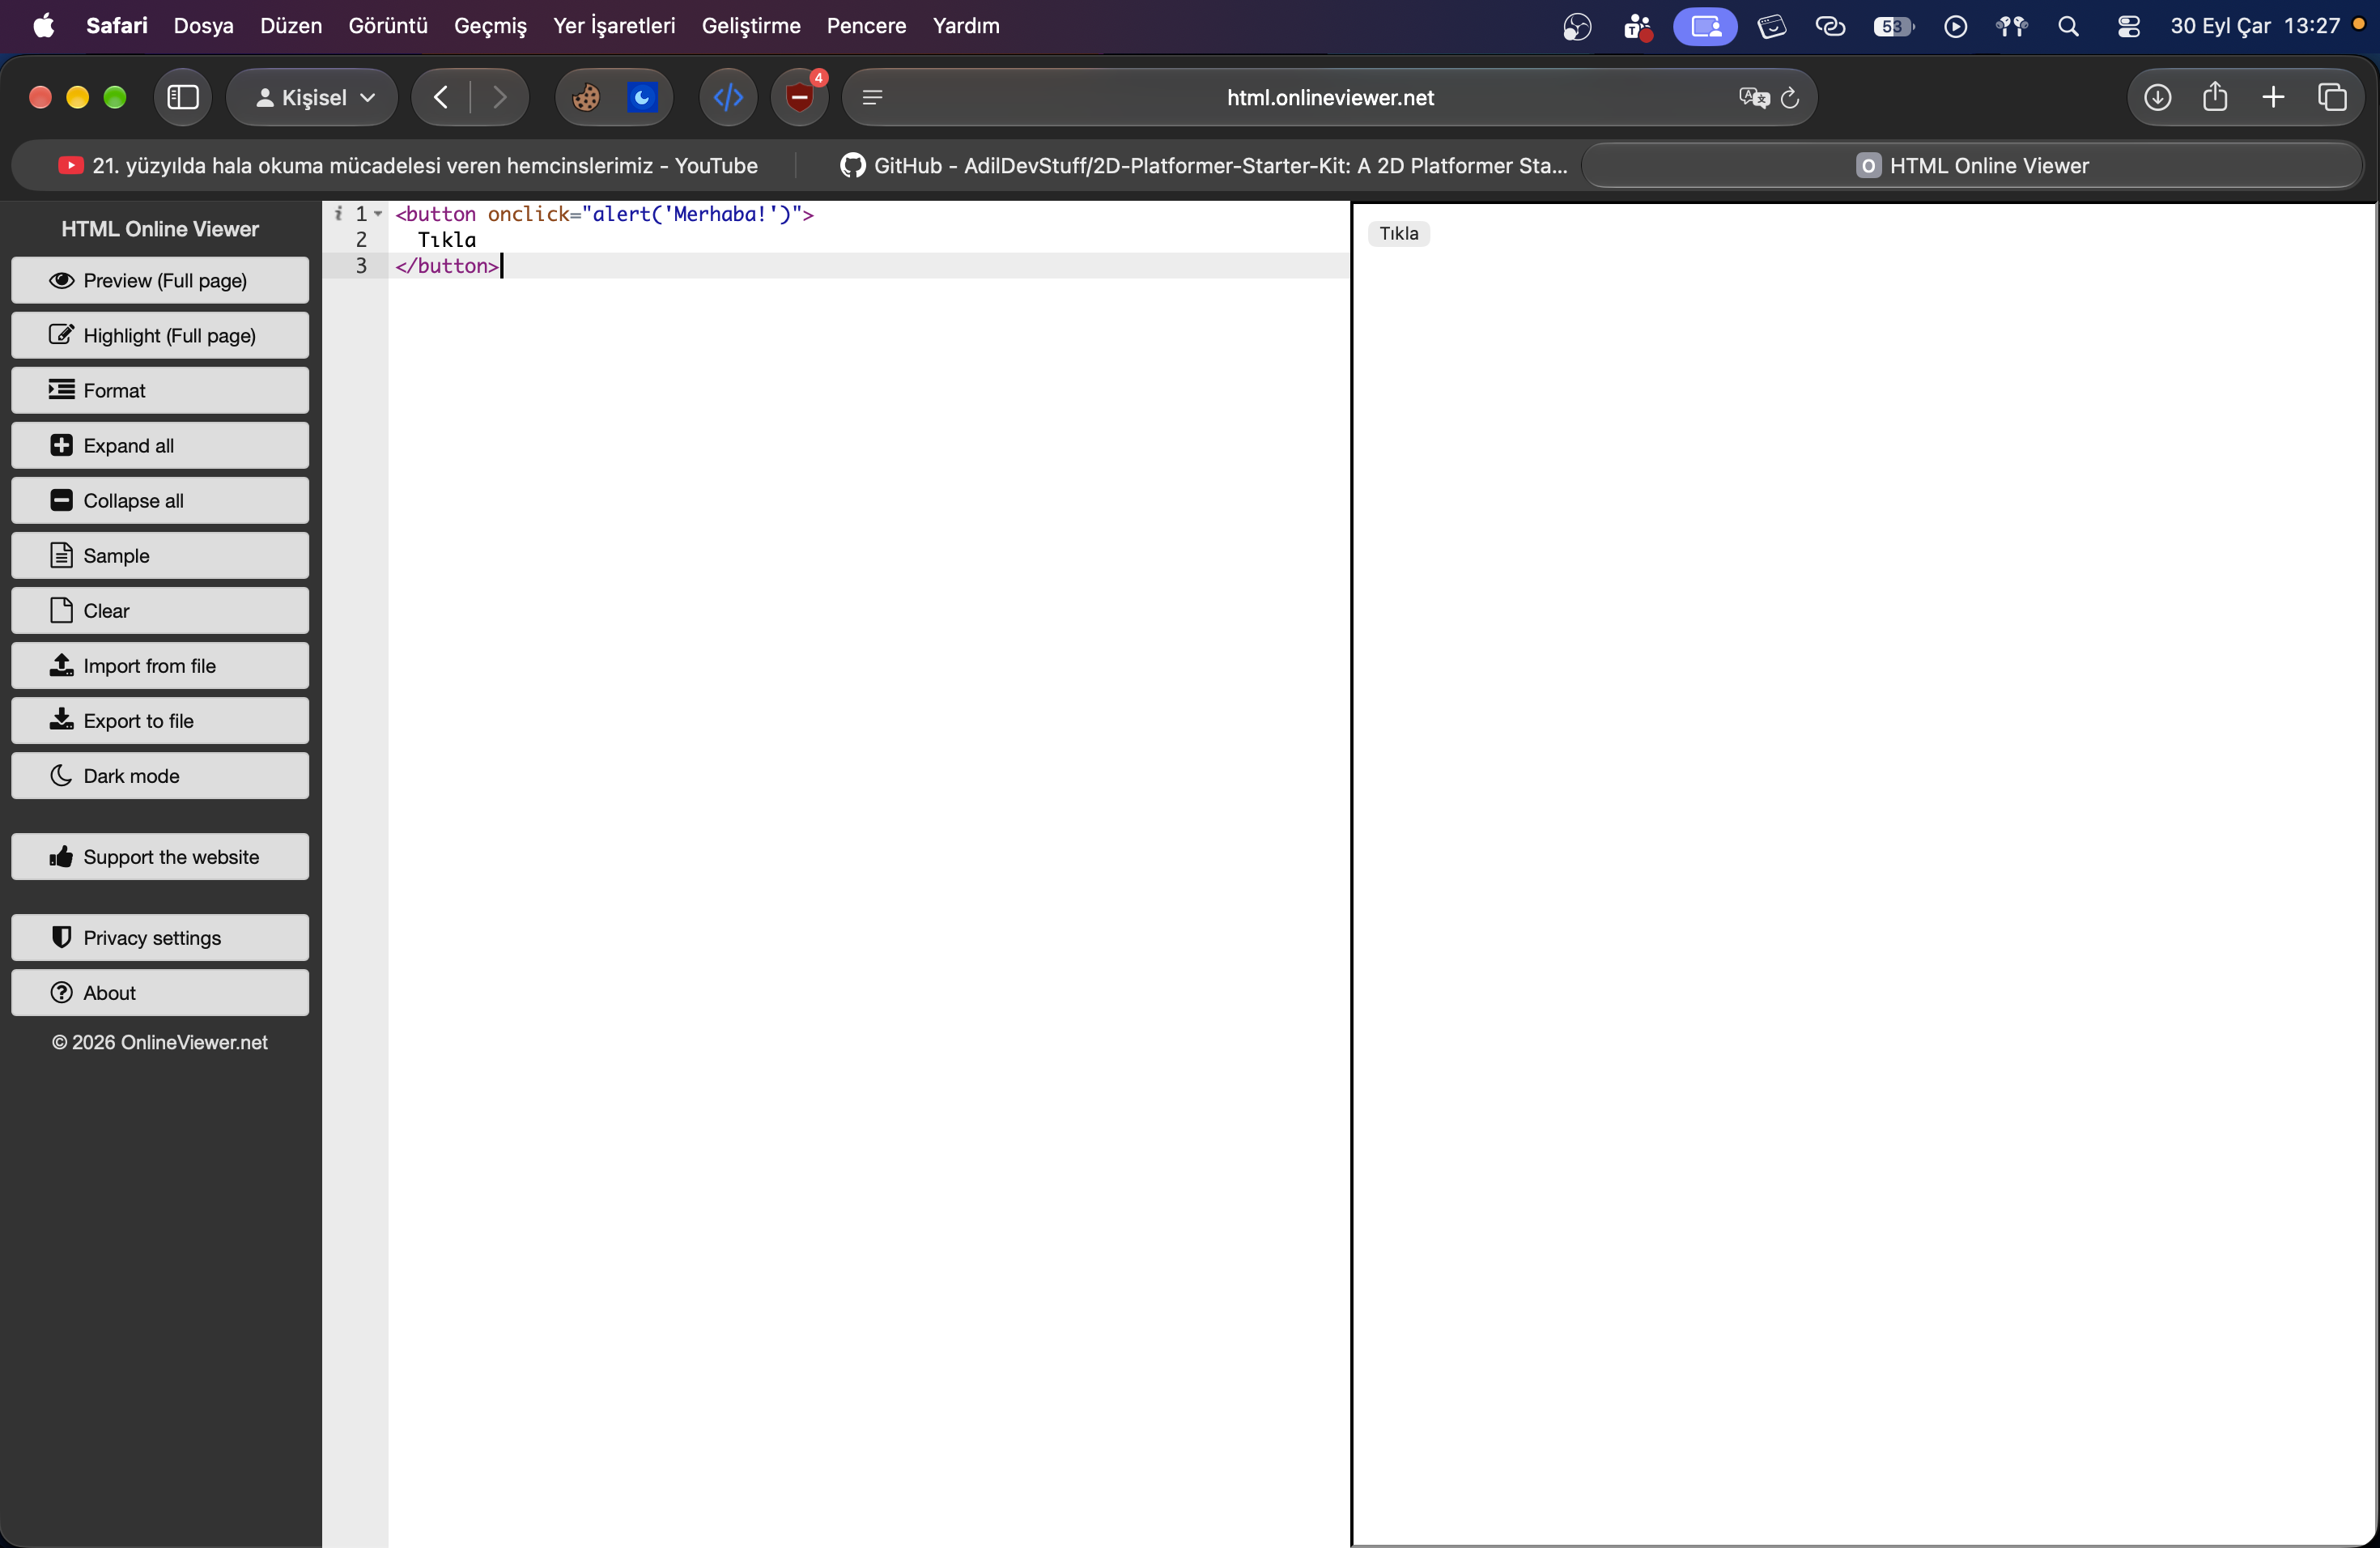
\includegraphics[width=\linewidth,height=.65\textheight,keepaspectratio]{eylul30-ilk.png}
\caption{30 Eylül: HTML onclick ile uyarı örneği.}
\end{figure}
\begin{figure}[p]
\centering
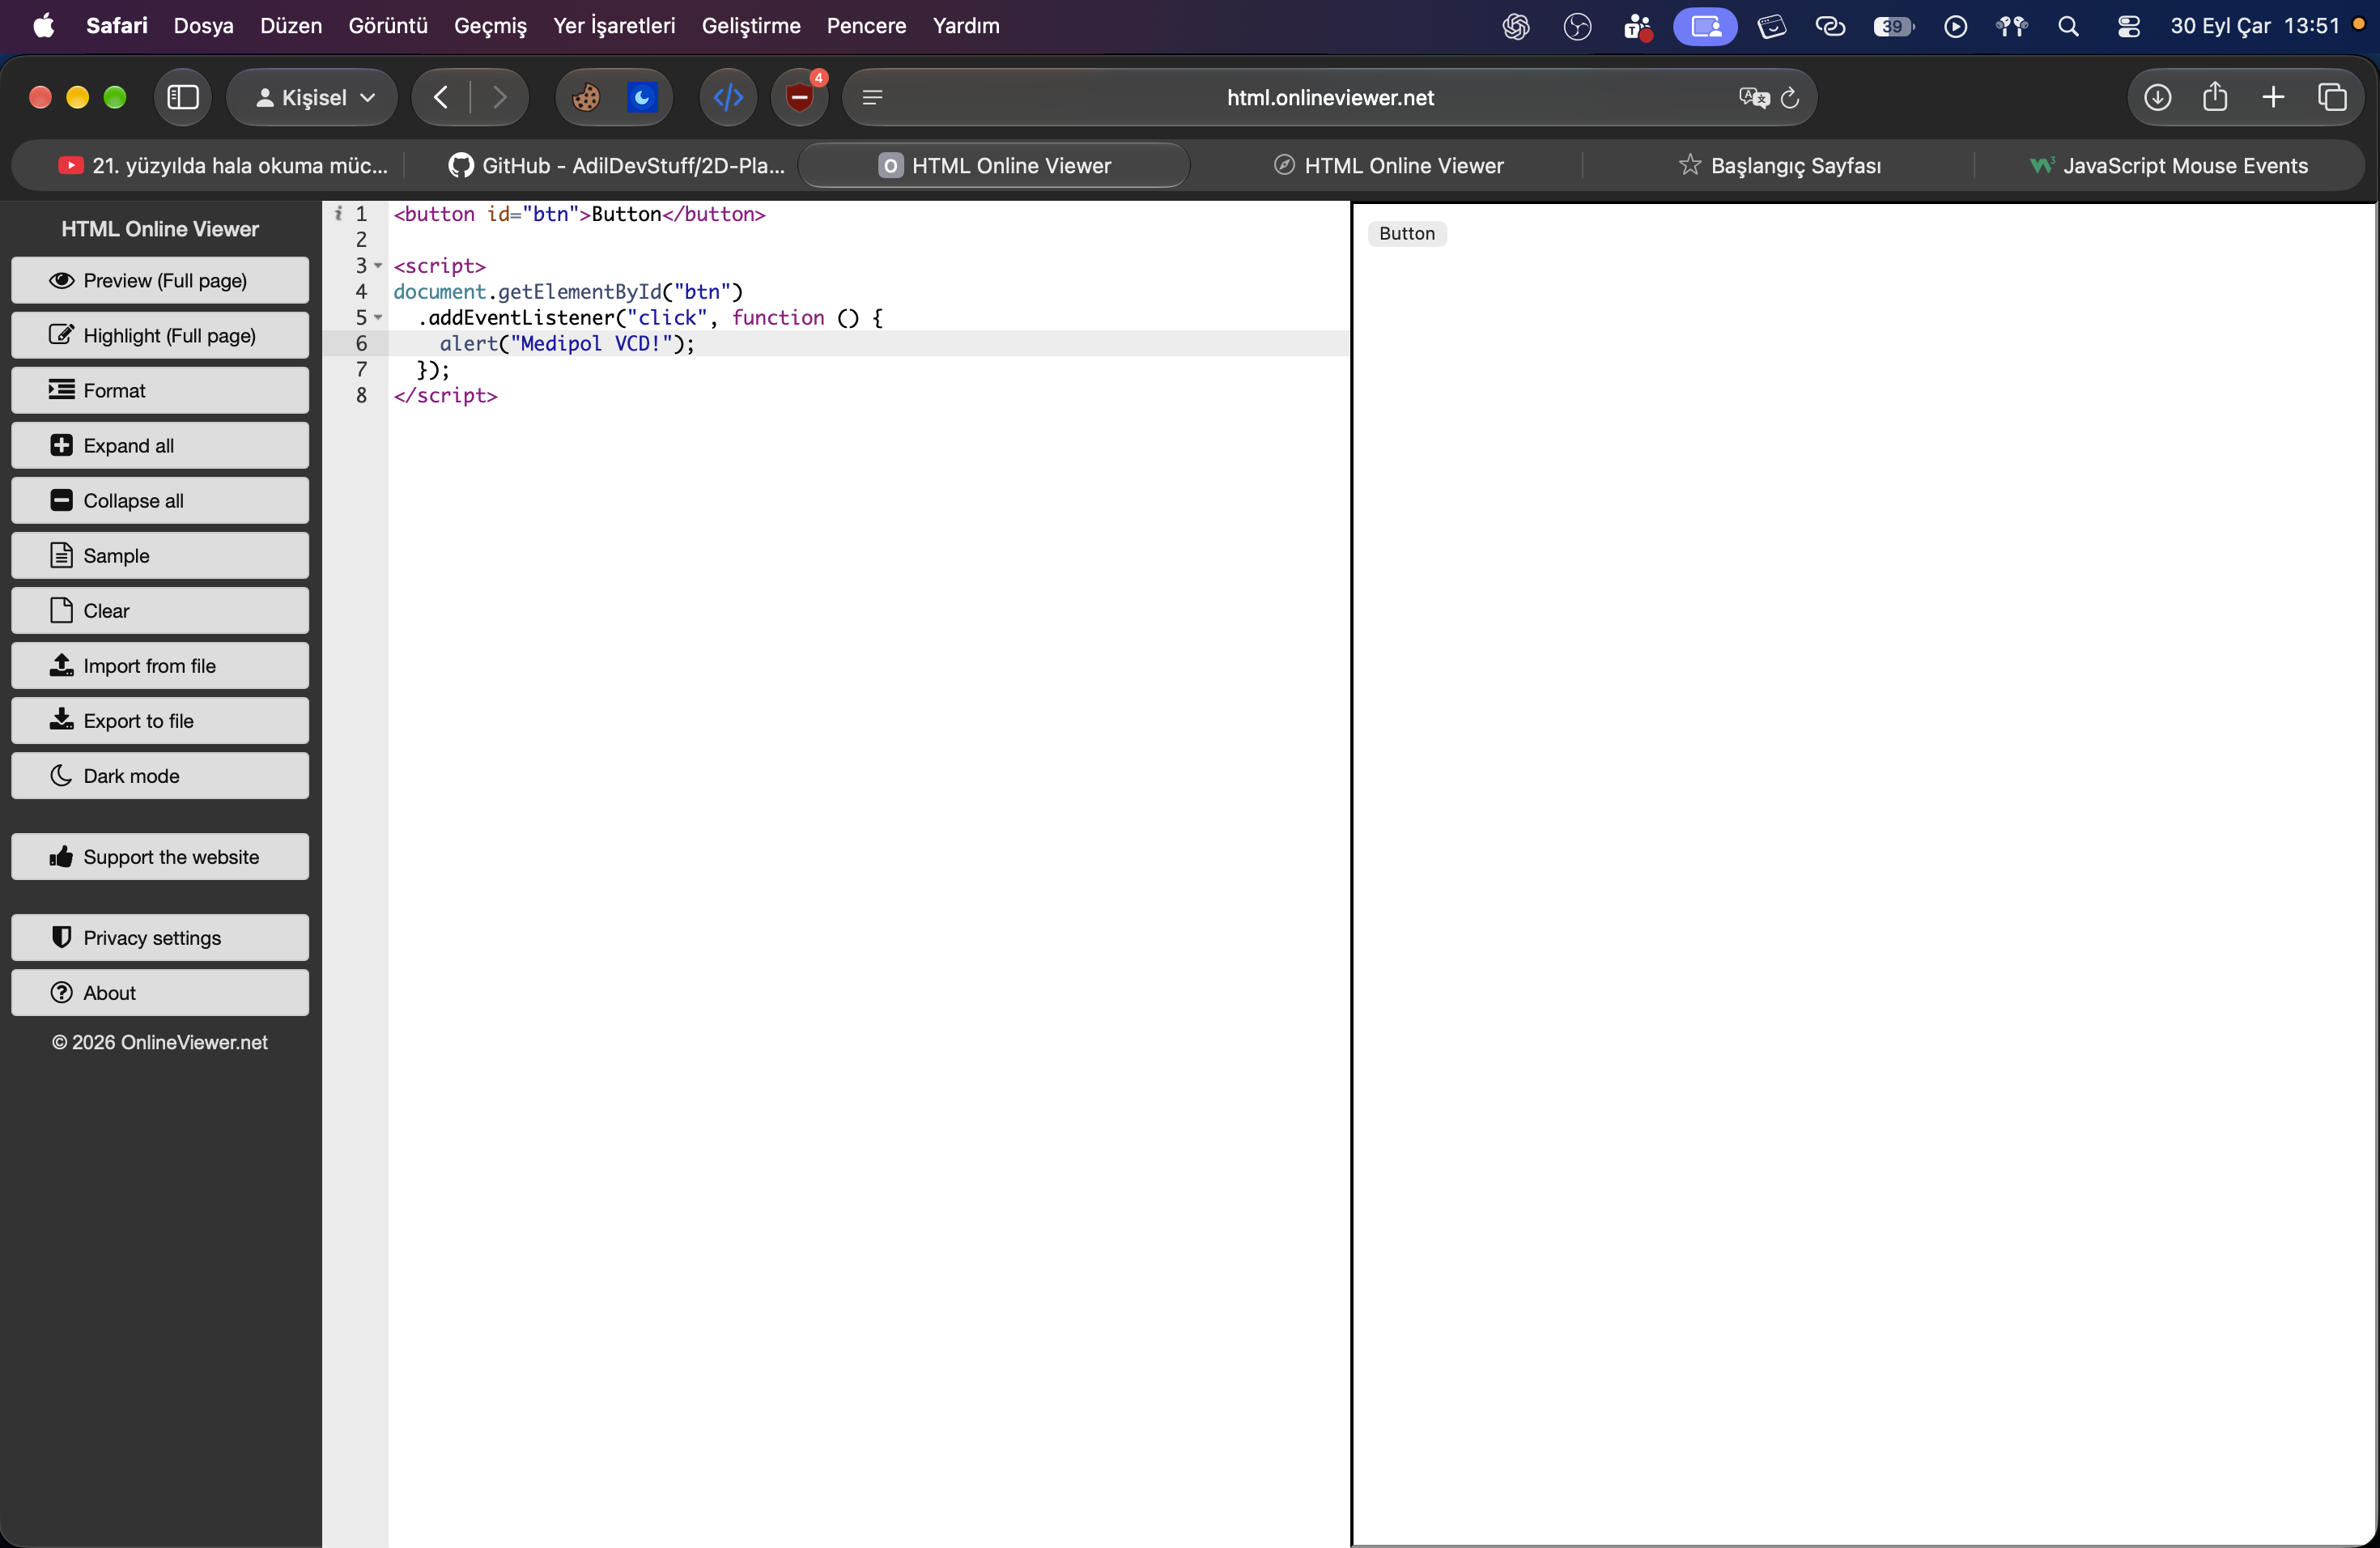
\includegraphics[width=\linewidth,height=.65\textheight,keepaspectratio]{eylul30-kod.png}
\caption{30 Eylül: addEventListener ile tıklama olayı.}
\end{figure}
\begin{figure}[p]
\centering
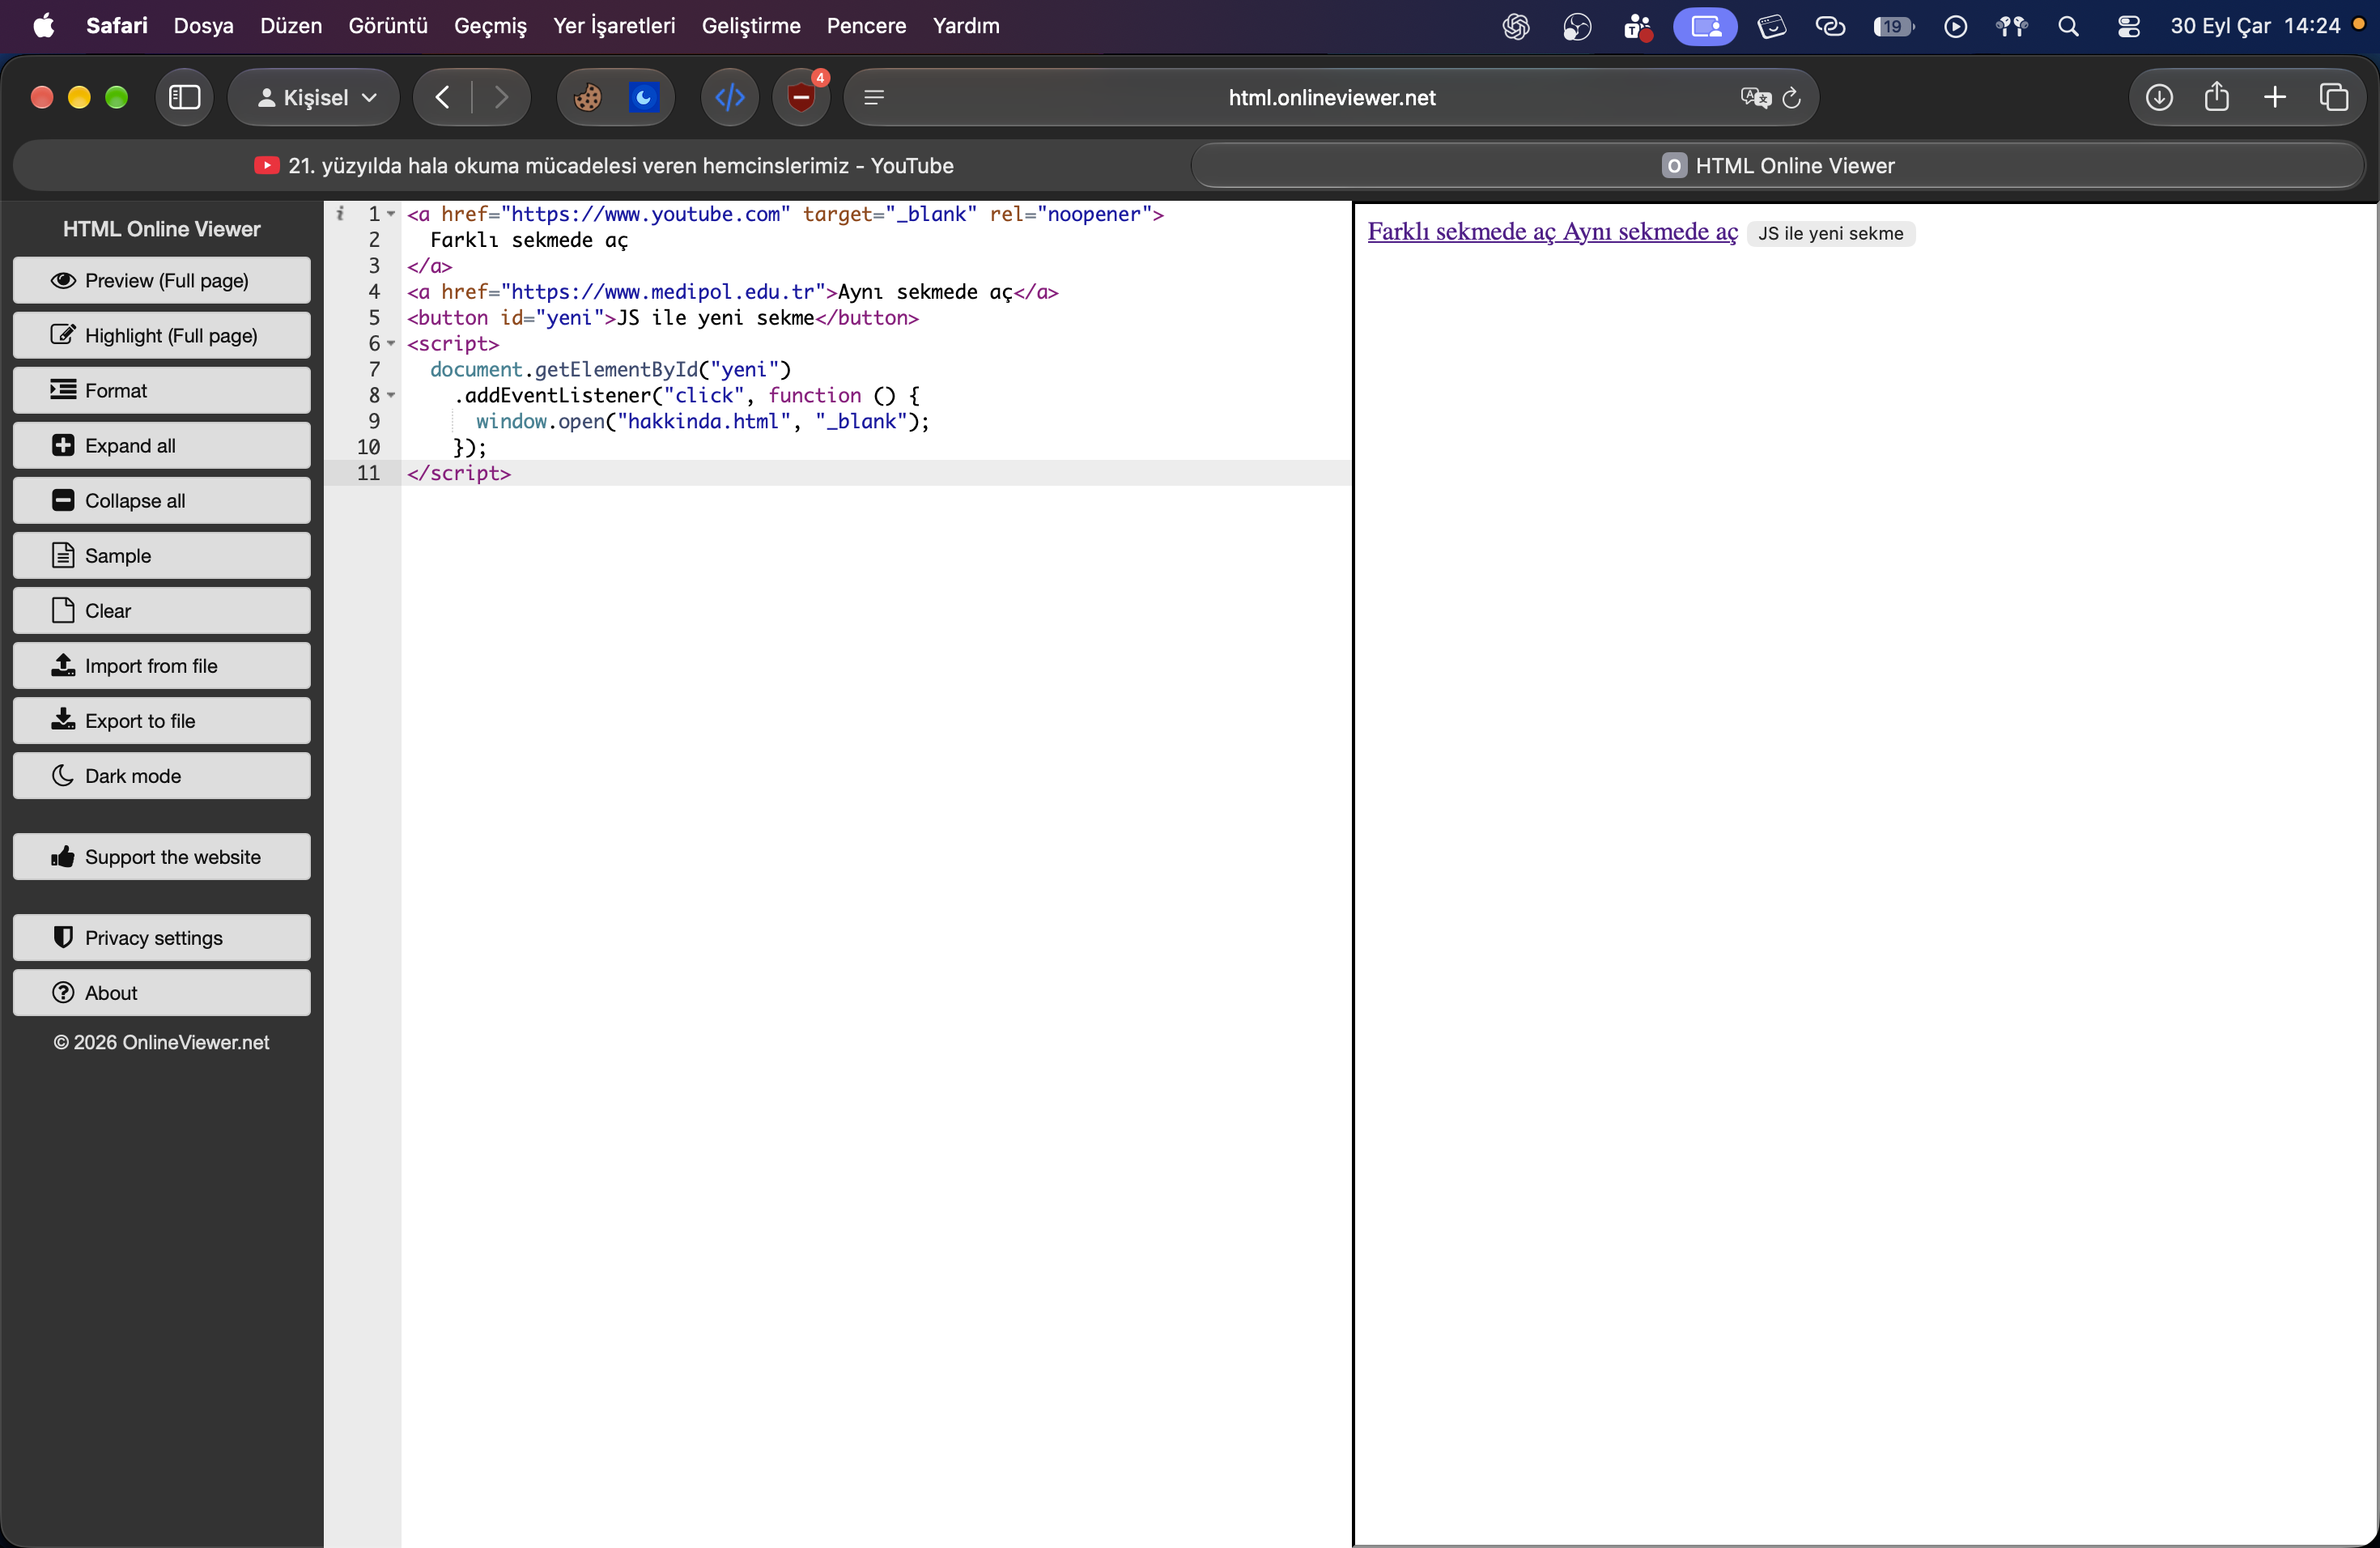
\includegraphics[width=\linewidth,height=.65\textheight,keepaspectratio]{eylul30-sekme.png}
\caption{30 Eylül: aynı sekme ve yeni sekme örnekleri.}
\end{figure}
\begin{figure}[p]
\centering
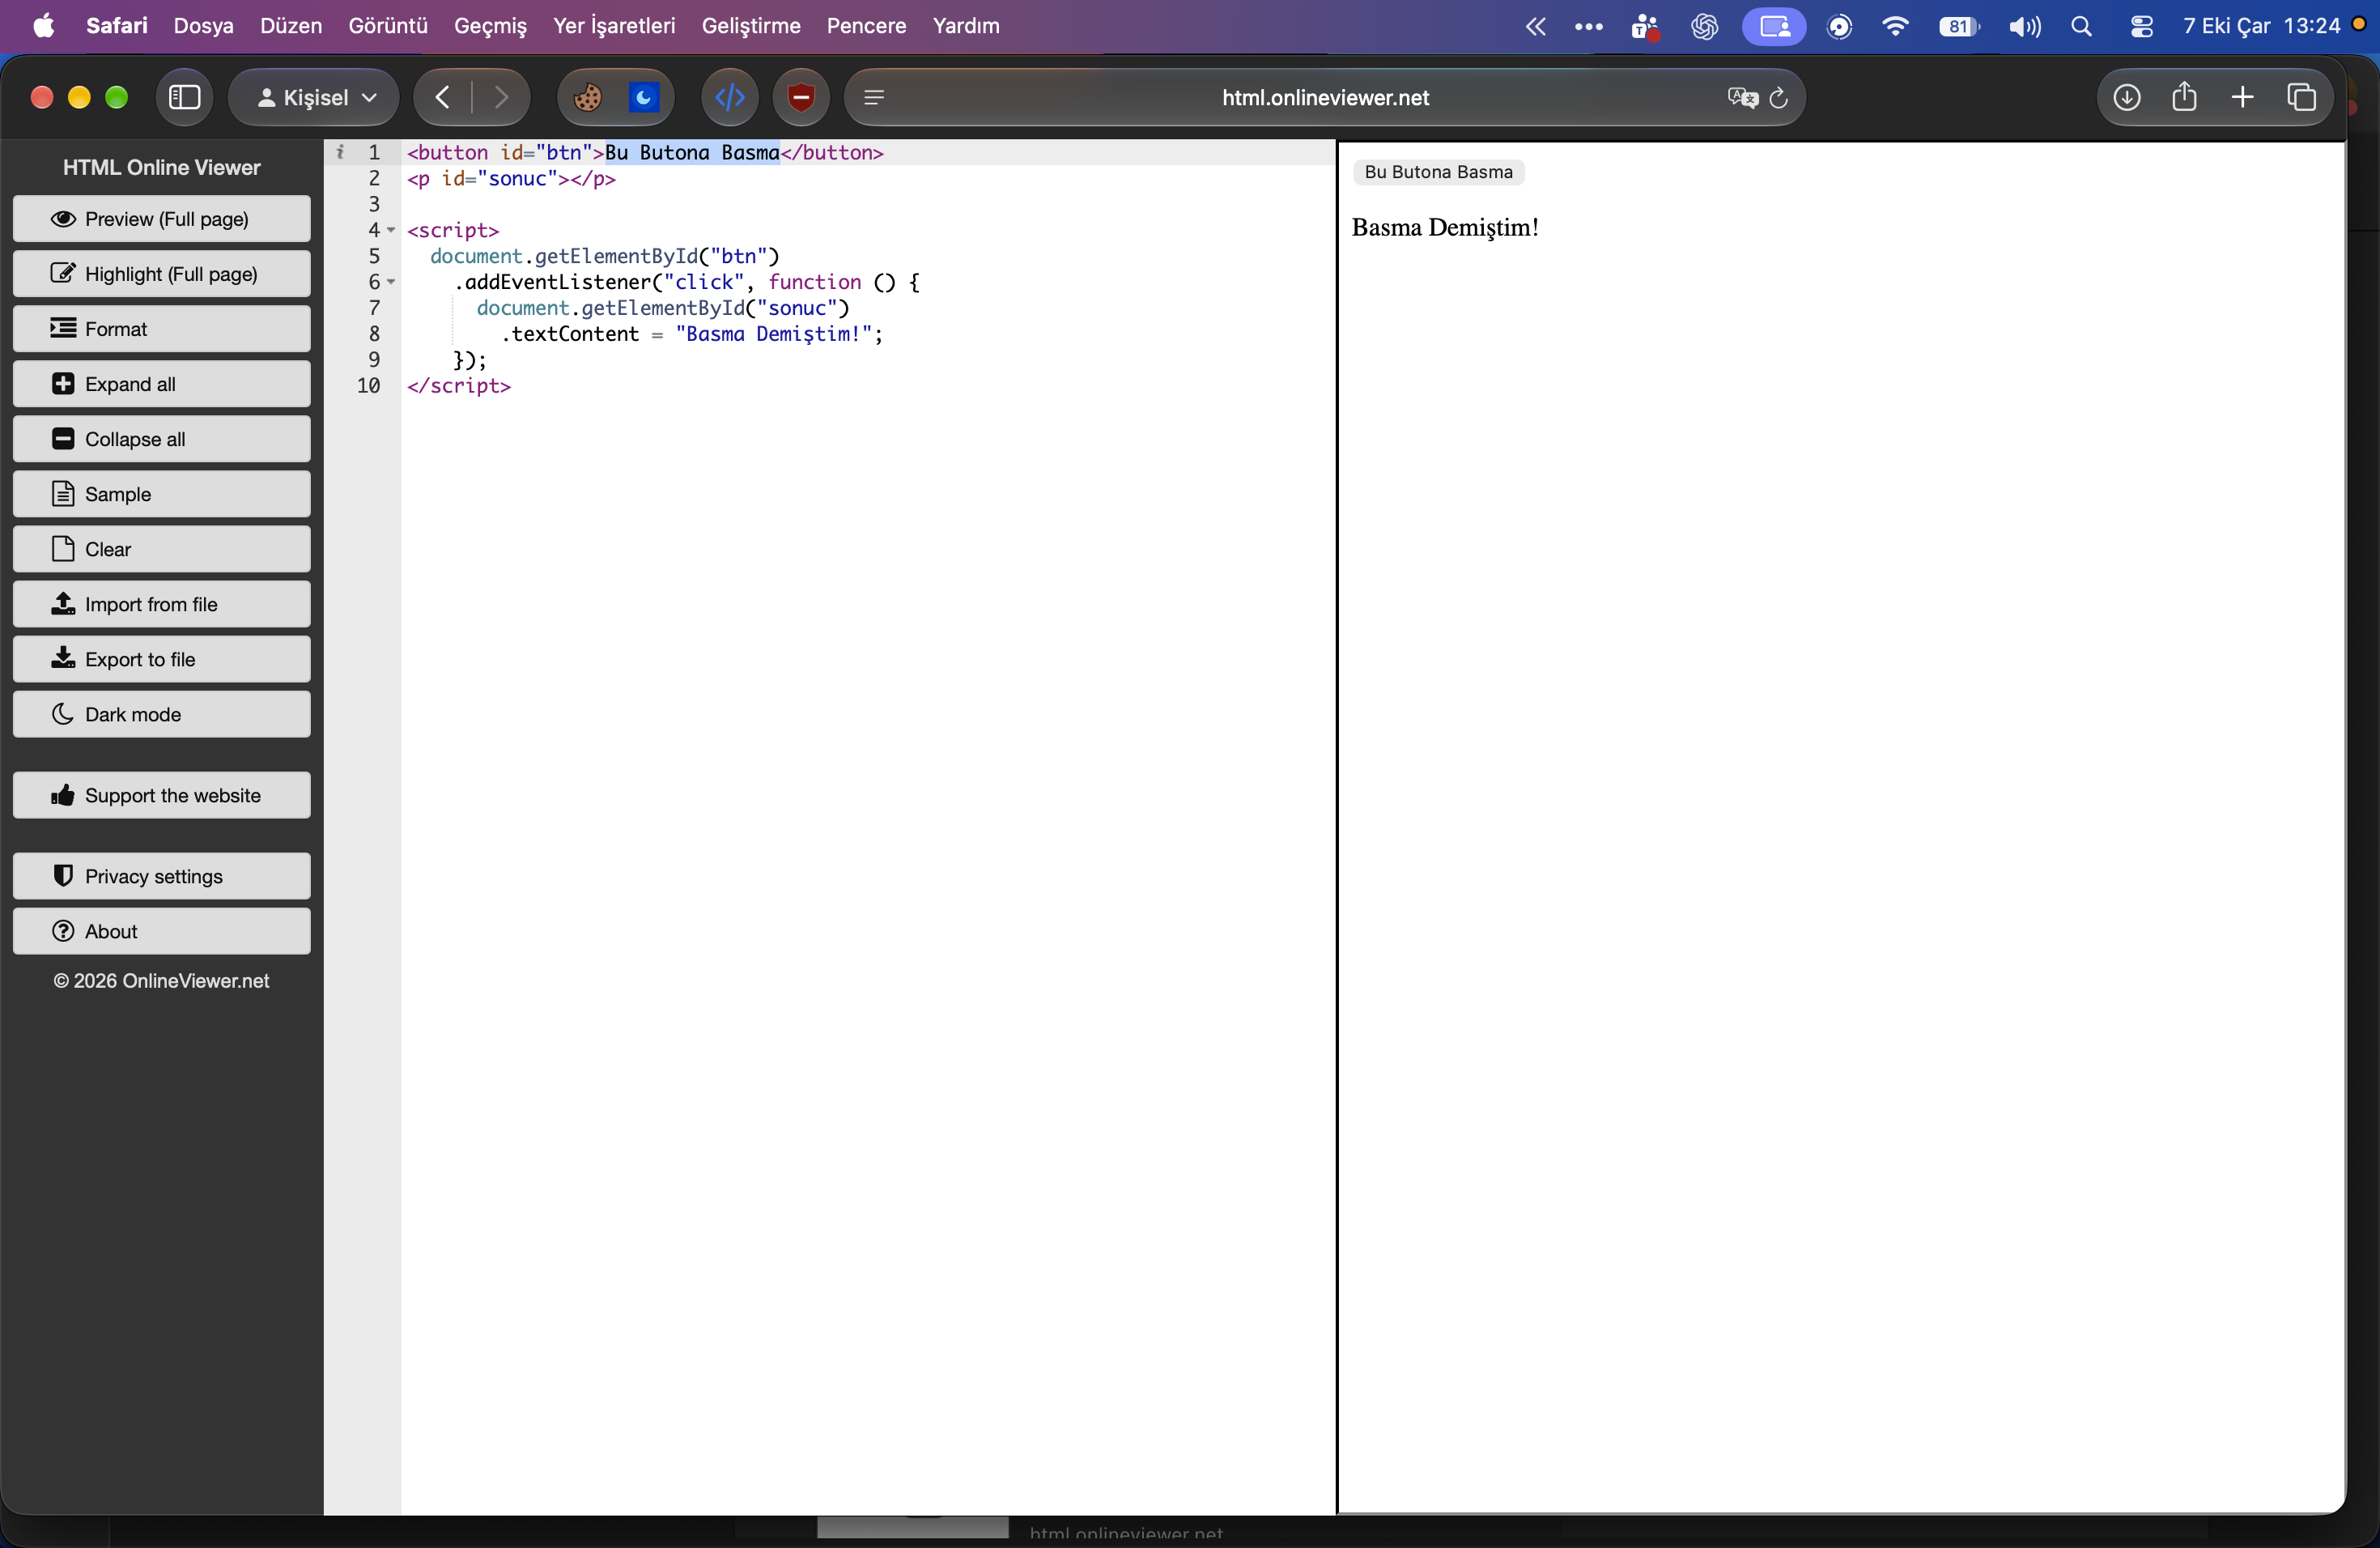
\includegraphics[width=\linewidth,height=.65\textheight,keepaspectratio]{ekim07-mesaj.png}
\caption{7 Ekim: tıklama ile metin güncelleme.}
\end{figure}
\begin{figure}[p]
\centering
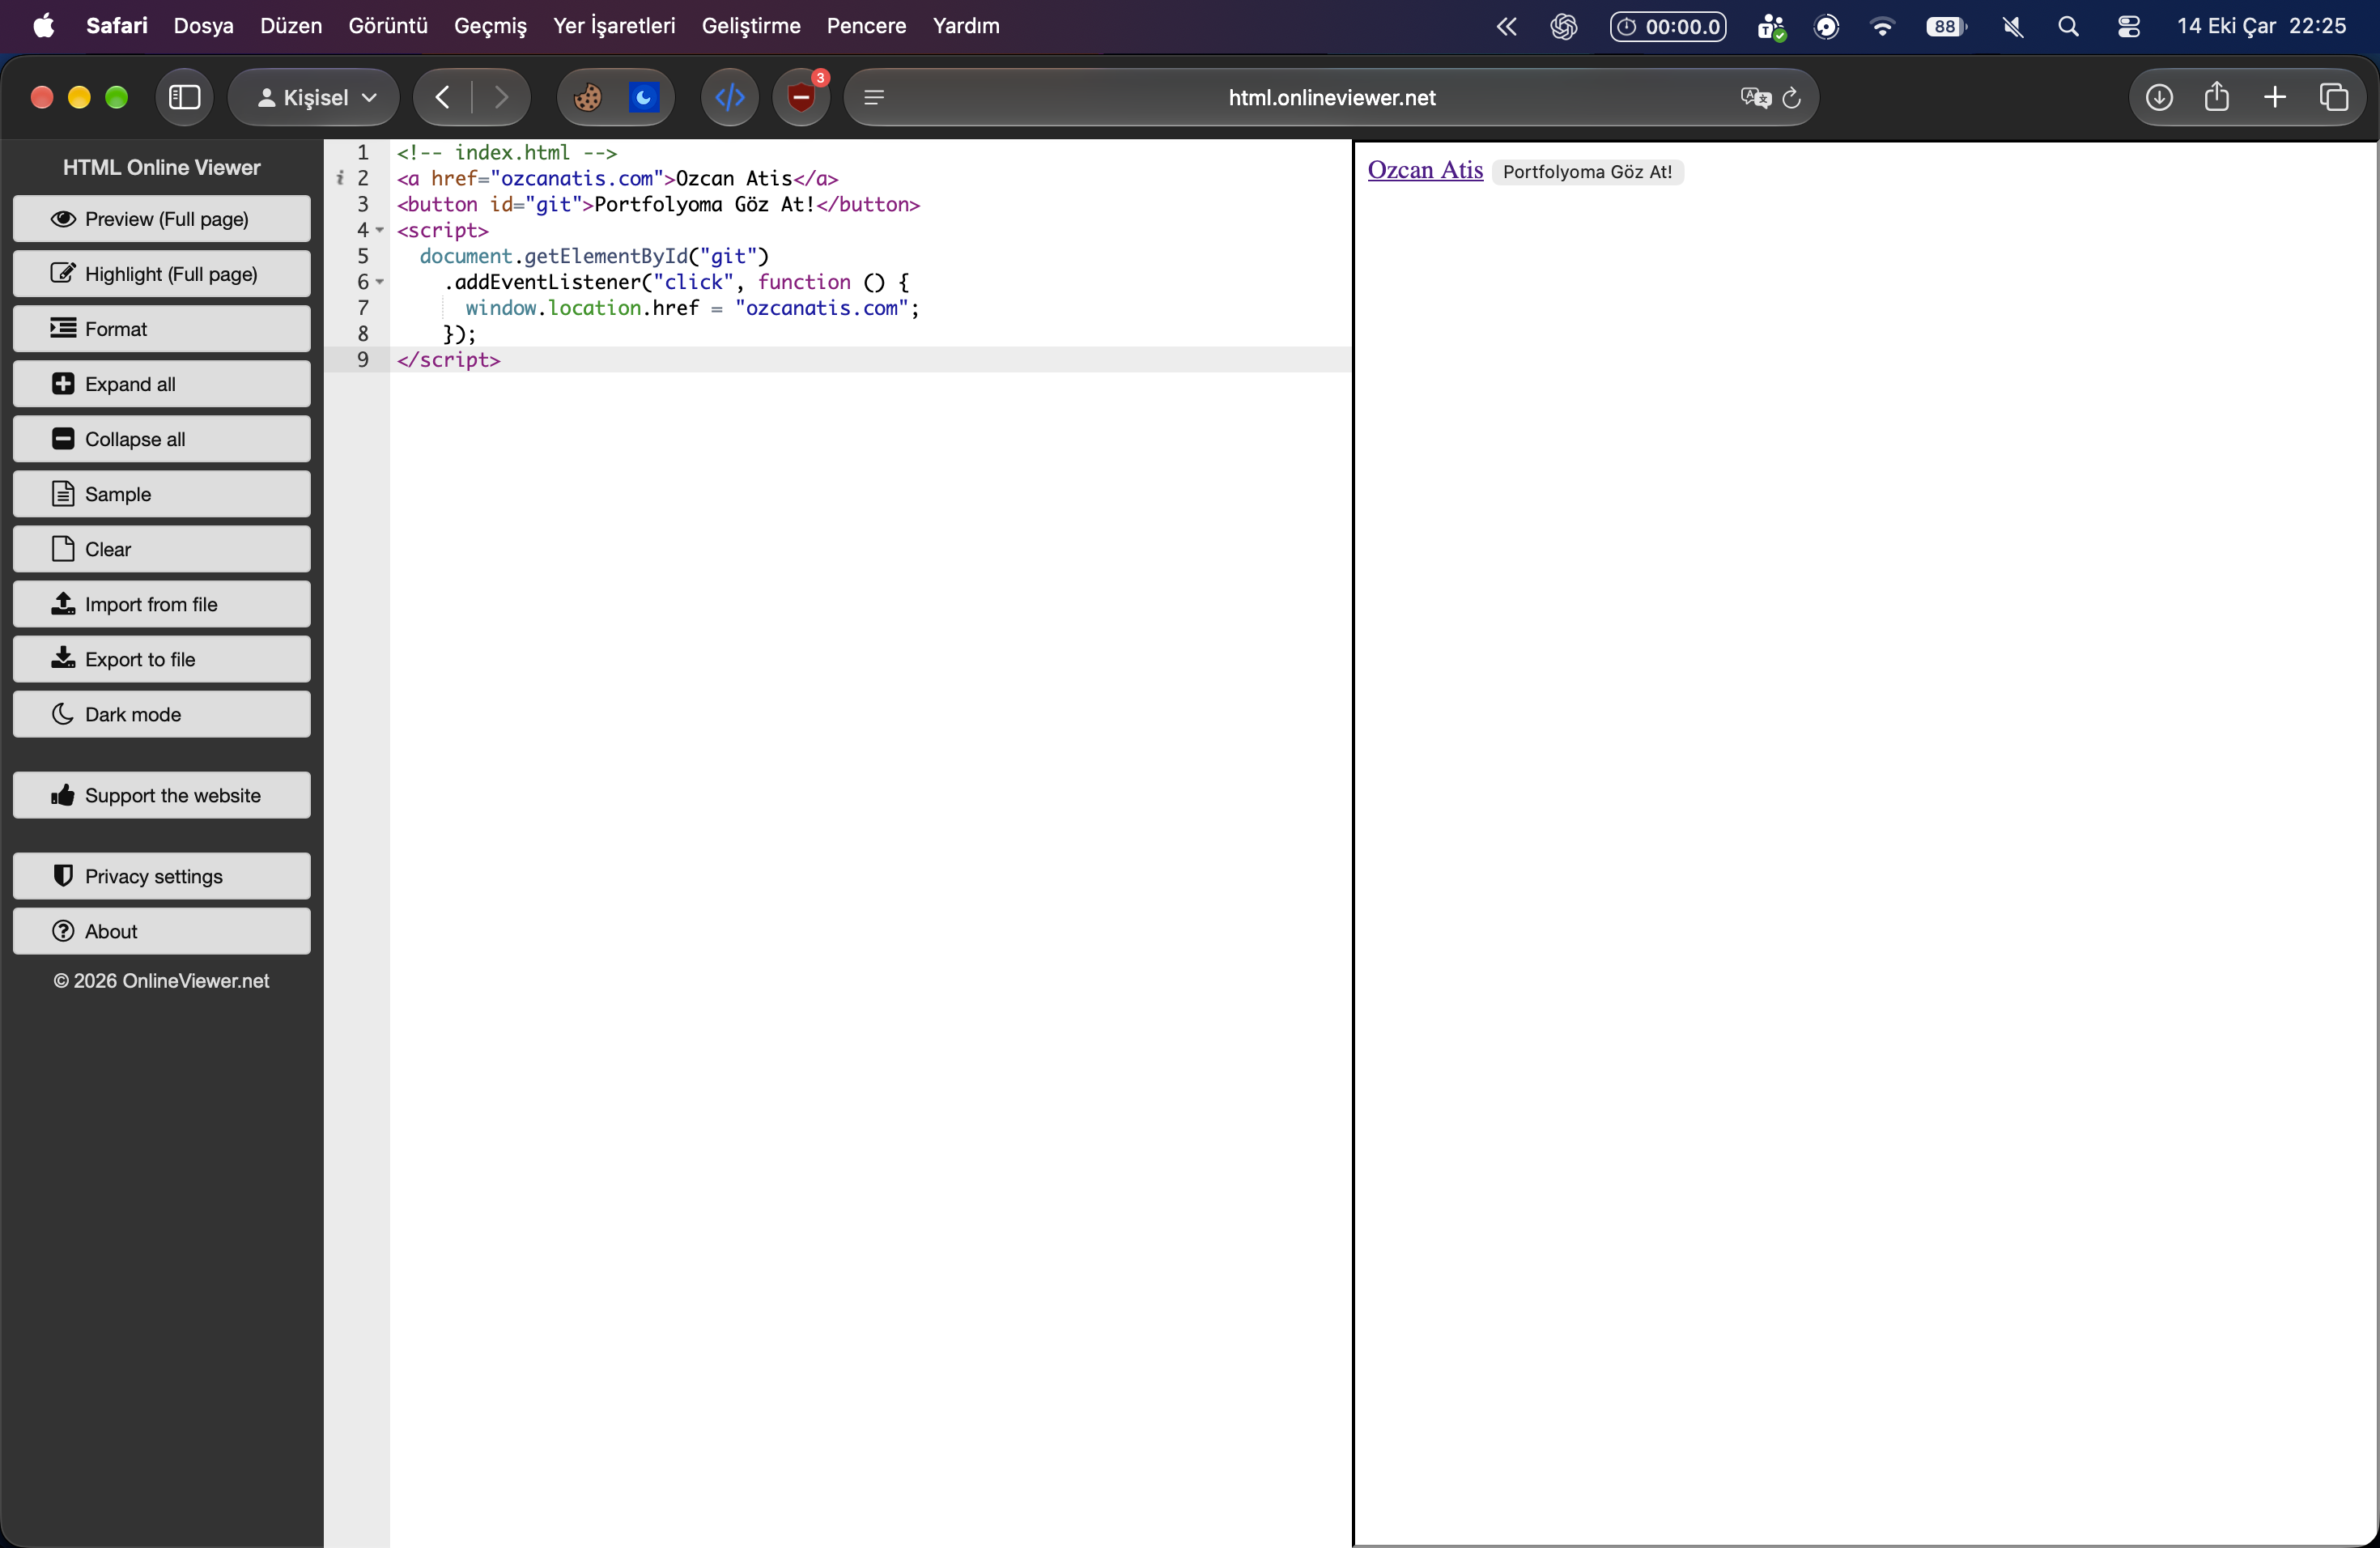
\includegraphics[width=\linewidth,height=.65\textheight,keepaspectratio]{ekim14-baglanti.png}
\caption{14 Ekim: bağlantı ve düğmeyle adres değiştirme.}
\end{figure}

\end{document}
